% conductor_rho_line_es -- edicion en castellano de conductor_rho_line.tex.
% 16 de septiembre de 2026.  Carles Marin + Claude (asistente IA).
%
% REGLA DE REDACCION: resultados, no proceso.  Lo que se dice de un tercero es lo que esta en un
% articulo suyo, con localizador.  Lo medido va marcado como medido, con su cifra y su rango.
% Traduccion fiel de la version inglesa; etiquetas, citas y matematicas identicas.
%
% Compilar:  pdflatex conductor_rho_line_es (x3).  Figuras: las versiones _es de figuras.py
\documentclass[11pt,a4paper]{article}
\usepackage[T1]{fontenc}
\usepackage[utf8]{inputenc}
\usepackage[spanish,es-noshorthands,es-nodecimaldot,es-tabla]{babel}
\usepackage{lmodern}
\usepackage[margin=2.6cm]{geometry}
\usepackage{amsmath,amssymb,amsthm}
\usepackage{graphicx}
\usepackage{booktabs}
\usepackage[dvipsnames,table]{xcolor}
\usepackage{float}
\usepackage[colorlinks=true,linkcolor=NavyBlue,citecolor=NavyBlue,urlcolor=NavyBlue,pagebackref=true,
  bookmarksnumbered=true,bookmarksopen=true]{hyperref}
\hypersetup{pdftitle={Donde los valores de los caracteres de Sp(2m) en un elemento de torsion no generan el anillo de enteros},
  pdfauthor={Carles Mar\'in}}
% cada referencia de la bibliografia enlaza a las paginas donde se cita
\renewcommand*{\backref}[1]{}
\renewcommand*{\backreftwosep}{ y~}
\renewcommand*{\backreflastsep}{ y~}
\renewcommand*{\backrefalt}[4]{{\footnotesize\textcolor{gray}{\ifcase #1 \or citado en la p\'agina~#2.\else citado en
  las p\'aginas~#2.\fi}}}
\usepackage{microtype}
\usepackage{needspace}
\renewcommand{\textfraction}{0.07}
\renewcommand{\topfraction}{0.92}
\renewcommand{\bottomfraction}{0.92}
\renewcommand{\floatpagefraction}{0.78}

\definecolor{azul}{HTML}{1F4E79}
\definecolor{fondoficha}{HTML}{EEF3F8}
\definecolor{filaclara}{HTML}{F2F6FA}

\newtheorem{theorem}{Teorema}
\newtheorem{proposition}[theorem]{Proposición}
\newtheorem{corollary}[theorem]{Corolario}
\newtheorem{lemma}[theorem]{Lema}
\theoremstyle{definition}
\newtheorem{observation}[theorem]{Observación}
\newtheorem{question}[theorem]{Pregunta}
\newtheorem{remark}[theorem]{Comentario}

\newcommand{\Sp}{\mathrm{Sp}}
\newcommand{\ZZ}{\mathbb{Z}}
\newcommand{\QQ}{\mathbb{Q}}
\newcommand{\FF}{\mathbb{F}}
\newcommand{\cO}{\mathcal{O}}
\newcommand{\cf}{\mathfrak{f}}
\newcommand{\rad}{\mathfrak{r}}
\newcommand{\gr}{\operatorname{gr}}
\newcommand{\pregunta}[1]{\par\smallskip\noindent\emph{#1}\par\smallskip}
% pregunta de frontera al cierre de una seccion: discreta, sin cifras
\definecolor{azulpregunta}{HTML}{1F6FB2}
\newcommand{\frontera}[1]{\par\medskip\noindent{\small\color{azulpregunta}$\triangleright$\ \emph{#1}}\par}
% formula clave: enmarcada, numerada y enlazable
\newcommand{\marco}[1]{{\setlength{\fboxsep}{6pt}\setlength{\fboxrule}{0.6pt}%
  \fcolorbox{azul!45}{fondoficha}{$\displaystyle #1$}}}

\newsavebox{\fichabox}
\newenvironment{keybox}
  {\par\vspace{9pt}\begin{lrbox}{\fichabox}%
   \begin{minipage}{0.90\textwidth}\vspace{7pt}\setlength{\parskip}{3pt}}
  {\vspace{7pt}\end{minipage}\end{lrbox}%
   \par\needspace{\dimexpr\ht\fichabox+\dp\fichabox+12pt\relax}\noindent\hbox to \textwidth{\hfill
   \textcolor{azul}{\rule[-\dp\fichabox]{3.2pt}{\dimexpr\ht\fichabox+\dp\fichabox\relax}}%
   \colorbox{fondoficha}{\usebox{\fichabox}}\hfill}%
   \par\vspace{9pt}}

\title{\vspace{-1.4cm}\Large Dónde los valores de los caracteres de $\Sp(2m)$ en un elemento de torsión\\
no generan el anillo de enteros}
\author{\normalsize Carles Mar\'in\thanks{Investigador independiente, \texttt{karlesmarin@gmail.com}.
El autor utilizó Claude (Anthropic) como asistente de investigación, comprobó cada afirmación y asume toda la
responsabilidad sobre el contenido de esta nota.}}
\date{\normalsize 16 de septiembre de 2026}

\begin{document}
\maketitle
\thispagestyle{empty}\enlargethispage{2pt}

\begin{abstract}
\noindent Sea $g\in\Sp(2m)$ con valores propios $\xi_q^{\pm1},\dots,\xi_q^{\pm m}$, con $1\le m<q/2$. Los valores de
todos los caracteres de $\Sp(2m)$ en $g$ generan un subanillo $A$ del anillo de enteros $\cO$ de $\QQ(\xi_q)^+$ que,
salvo en casos conocidos en los que es $\ZZ$, es un orden. Localizamos y describimos su conductor. Escribimos $h=2m$ y
$q=p^vq'$ con $p\nmid q'$. Todo primo del índice $[\cO:A]$ divide a $q$, y para $q'\notin\{1,2,3,4,6\}$ un primo
$p\mid q$ lo divide si y solo si $q'$ divide a $h$, $h+1$ o $h+2$. En cada primo el conductor es una potencia del
radical. En un tal $p$ con $\varphi(p^v)\ge2$, la primera capa graduada de $A$ tiene la dimensión del módulo cíclico
sobre $\FF_p[(\ZZ/q')^\times]$ generado por una función de primer momento $S$ explícita, y decide si esa potencia es
$1$ y, cuando es $2$, ambas longitudes y si el anillo local es de Gorenstein. Para $p$ impar y
$q'\notin\{1,2,3,4,6\}$, los segmentos estables dan a $S$ dos formas: el diente de sierra de Stickelberger cuando
$m\equiv0,-1\pmod{q'}$, y ese mismo diente desplazado medio periodo cuando $2m+1=Nq'$ o cuando $q'$ es par y
$m\equiv q'/2,q'/2-1\pmod{q'}$. En las familias del diente y en las de medio periodo con $q'$ par, una identidad de
medio periodo y un lema de duplicación las ponen en un mismo retículo, y la fórmula del
índice de Sinnott calcula la parte $p$ de los menores
maximales de la matriz de momentos: el conductor en $p$ es el radical exactamente cuando $p$ no divide a
$h^-(\QQ(\zeta_{q'}))$, y un divisor simple de $h^-$ da el cuadrado del radical en $p$ y un anillo local de Gorenstein.
Cuando en cambio $2m+1=Nq'$ y $p\nmid N\,h^-$, la primera capa, ambas longitudes y el tipo de Cohen--Macaulay se leen
en el subgrupo generado por $2$ en $(\ZZ/q')^\times$. Siempre que esa primera capa, de dimensión $w$, esté más que
medio llena, el índice en $p$ queda cerrado: $v_p([\cO:A])=2d-1-w$, con $d=\varphi(q')/2$ la dimensión del anillo
residual. Las respuestas reúnen el conductor de Dedekind, el vínculo de Kummer
entre los números de Bernoulli y los números de clase, y la combinatoria de las escalas musicales.
\end{abstract}

\medskip
\noindent\textbf{Palabras clave:} valores de caracteres; órdenes en cuerpos ciclotómicos; conductor; ideal de
Stickelberger; anillo de Gorenstein; número de clase relativo.

% ==============================================================================================
\section{De qué trata esta nota}\label{sec:intro}

Un carácter de un grupo de Lie compacto, evaluado en un elemento de orden finito, es un entero algebraico.
Tomemos todos los caracteres a la vez, en un mismo elemento: generan un anillo. Para el elemento
$g=g_{1/q}\in\Sp(2m)$ con valores propios $\xi_q^{\pm j}$, $1\le j\le m$, ese anillo vive dentro del anillo de
enteros $\cO=\ZZ[\xi_q+\xi_q^{-1}]$ del cuerpo ciclotómico real. De ahí salen dos preguntas, una dentro de la
otra:

\pregunta{¿Generan los valores de los caracteres el anillo de enteros? Y donde no lo hacen, ¿qué falta
exactamente?}

\noindent Ambas preguntas son más antiguas que el anillo. En 1877, contando clases de ideales en los órdenes de un
cuerpo de números, Dedekind asoció a cada orden el mayor ideal del orden maximal que está contenido en él, su
\emph{Führer}, o conductor \cite{Ded77}. Un año después mostró que, sobre un primo $p$ que no divide al índice
$[\cO:\ZZ[\alpha]]$, los primos de $\cO$ se leen en la factorización módulo $p$ del polinomio mínimo de $\alpha$
\cite{Ded78}. Qué primos dividen al índice, y cómo es el conductor en cada uno de ellos, han sido desde entonces lo
primero que se pregunta sobre un orden. Lo que cambia aquí es quién elige los generadores: no un número $\alpha$,
sino todos los caracteres irreducibles de $\Sp(2m)$, evaluados a la vez en $g$.

\noindent La primera pregunta tiene una respuesta limpia, y la respuesta a la segunda resulta estar escrita en
tres lenguajes más antiguos: la combinatoria de las escalas musicales, el formalismo de longitudes de los anillos
de dimensión uno y la aritmética de los números de Bernoulli. La nota se organiza como una sucesión de preguntas,
cada una planteada por la respuesta a la anterior. La Figura~\ref{fig:estructura} dibuja ese hilo, y la tabla
recoge las respuestas.

\begin{figure}[htbp]
\centering
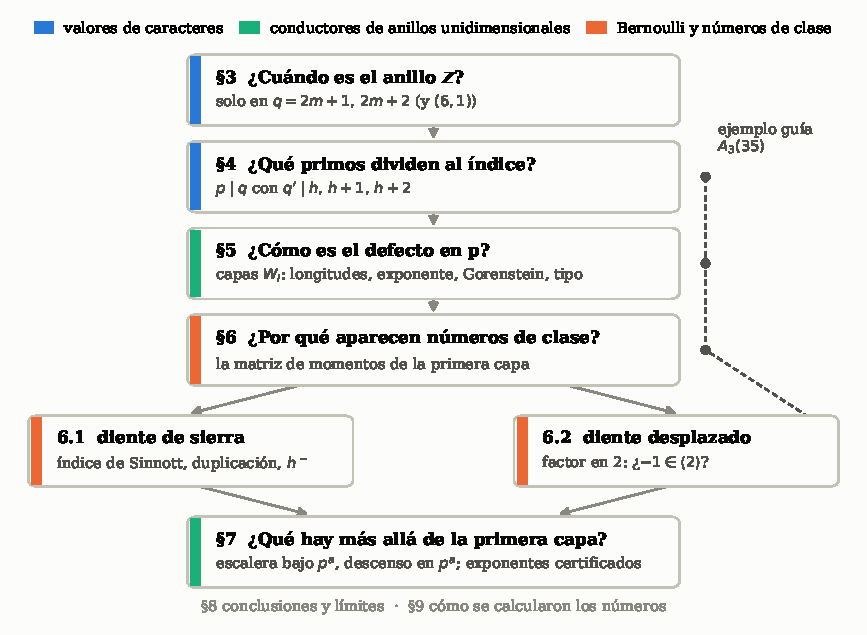
\includegraphics[width=0.94\textwidth]{fig_estructura_es.pdf}
\caption{El hilo de la nota. Cada sección responde a la pregunta que deja la de encima; en el \S\ref{sec:clase} los
dos tipos de segmento estable parten la respuesta en dos. El color de cada caja indica en cuál de las tres líneas del
\S\ref{sec:historia} se apoya, y la línea discontinua sigue el ejemplo guía $A_3(35)$.}
\label{fig:estructura}
\end{figure}

\medskip
\begin{center}\small
\rowcolors{2}{filaclara}{white}
\begin{tabular}{p{0.44\textwidth}p{0.47\textwidth}}
\toprule
pregunta & respuesta \\
\midrule
¿Cuándo es el anillo simplemente $\ZZ$? (\S\ref{sec:set}) & exactamente en los puntos enteros de una nota anterior: Proposición~\ref{prop:AZ} \\
¿Qué primos dividen al índice? (\S\ref{sec:sop}) & solo primos de $q$; y, para $q'\notin\{1,2,3,4,6\}$, $p\mid[\cO:A]$ si y solo si la parte $q'$, prima con $p$, del orden de $g$ divide a $h$, $h+1$ o $h+2$: Teorema~\ref{thm:sop}, Figura~\ref{fig:paisaje} \\
¿Cómo es el defecto en un primo? (\S\ref{sec:loc}) & un único cuerpo residual $\FF_p$, una primera capa medida por un módulo cíclico, longitudes como sumas de los defectos de las capas, un criterio de Gorenstein y el tipo de Cohen--Macaulay: Teorema~\ref{thm:loc}, Proposiciones~\ref{prop:cert}--\ref{prop:tipo} \\
¿Por qué aparecen números de clase? (\S\ref{sec:clase}) & los menores maximales de la matriz de momentos son el índice de Sinnott (salvo una potencia de $2$ si $q'\equiv2\pmod4$), así que $h^-$ decide si la primera capa está llena; para $2m+1=Nq'$ y $p\nmid N\,h^-$ lo decide el subgrupo $\langle2\rangle$: Proposición~\ref{prop:sinnott}, Lema~\ref{lem:dobla}, Teorema~\ref{thm:hminus}, Corolarios~\ref{cor:simple}, \ref{cor:dos}, Figuras~\ref{fig:sierra}--\ref{fig:stickel} \\
¿Qué hay más allá de la primera capa? (\S\ref{sec:capas}) & una escalera universal por debajo de $p^{v_p(N)}$, descenso a un orden menor en $p^{v_p(N)}$, exponentes certificados por semigrupos, y una pregunta sobre lo que hay más allá: Proposiciones~\ref{prop:escalera}, \ref{prop:descenso}, Corolario~\ref{cor:semigrupo}, Figura~\ref{fig:perfil} \\
¿Qué está demostrado, y dónde se detiene? (\S\ref{sec:open}) & qué es nuestro, qué descansa en otros, qué solo se midió y qué no está cubierto \\
\bottomrule
\end{tabular}
\end{center}


\noindent\textbf{Un ejemplo guía.} Tomemos $m=3$ y $q=35$, de modo que $A=A_3(35)$ tiene rango $\varphi(35)/2=12$ y
$h=6$. En $p=7$, $q'=5$ no divide a ninguno de $6,7,8$; en $p=5$, $q'=7=h+1$. Así que solo $5$ divide al índice, y el
ejemplo se sigue a lo largo de los \S\S\ref{sec:sop}--\ref{sec:clase} hasta que $[\cO:A]=5^3$ y $\cf\,\cO_5=\rad^2$
salen a mano.

\medskip
\begin{center}\small
\rowcolors{2}{filaclara}{white}
\begin{tabular}{llp{0.62\textwidth}}
\toprule
símbolo & & significado \\
\midrule
$q$, $\xi$, $K$, $\cO$ & & orden de $g$; $\xi=\xi_q$; $K=\QQ(\xi)^+$; $\cO=\ZZ[\xi+\xi^{-1}]$ \\
$m$, $h$ & & rango; $h=2m$, el número de Coxeter de $C_m$ \\
$A$, $\cf$ & & el orden~\eqref{eq:A}; su conductor $(A:\cO)$ \\
$p$, $v$, $q'$, $E$ & & un primo; $q=p^vq'$, $p\nmid q'$; $E=\varphi(p^v)$, el índice de ramificación de $p$ en $K$ cuando $q'\ge3$ \\
$D$ & & $[K:\QQ]=\varphi(q)/2$; $D=Ed$ cuando $q'\ge3$ \\
$f$, $d$ & & grado residual de $p$ en $K$; $d=\varphi(q')/2=\dim_{\FF_p}\cO/\rad$ \\
$\rad$, $e=e_p$ & & radical de $\cO_p=\cO\otimes\ZZ_p$; $\cf\,\cO_p=\rad^{e}$ \\
$N^{(n)}$, $S$ & & el segmento $\{\pm1,\dots,\pm m\}$ contado módulo $n$; su primer momento~\eqref{eq:S} \\
$W_i$ & & $\dim_{\FF_p}$ de la $i$-ésima capa graduada de $A$ en $p$ \\
$N$ & & el cociente en $m=Nq'$, $m+1=Nq'$ o $2m+1=Nq'$ \\
\bottomrule
\end{tabular}
\end{center}

\noindent Los teoremas van en recuadros y las fórmulas clave, enmarcadas. Los enunciados que descansan en el
cálculo y no en una demostración llevan la etiqueta \emph{medido} u \emph{observado}, con la cuenta y el rango. En
un solo lugar, las respuestas dicen así.

\begin{keybox}
\noindent\textbf{Resultados principales.} Sea $A\ne\ZZ$, sea $p$ un primo, $q=p^vq'$ con $p\nmid q'$, $E=\varphi(p^v)$ y
$d=\varphi(q')/2$.
\begin{enumerate}
\item[(1)] \emph{Soporte} (Teorema~\ref{thm:sop}). Si $p\mid[\cO:A]$ entonces $p\mid q$; y si $p\mid q$ y
 $q'\notin\{1,2,3,4,6\}$, entonces $p\mid[\cO:A]$ si y solo si $q'$ divide a $h$, $h+1$ o $h+2$.
\item[(2)] \emph{Estructura local} (Lema~\ref{lem:galois}, Teorema~\ref{thm:loc}). $\cf\,\cO_p=\rad^{e_p}$. Si además
 $q'\notin\{1,2,3,4,6\}$, $E\ge2$ y $p\mid[\cO:A]$, entonces $W_1=\dim_{\FF_p}\FF_p[(\ZZ/q')^\times]\cdot S$ con $S$ como en~\eqref{eq:S}; $e_p=1$ si
 y solo si $W_1=d$; $v_p([\cO:A])=\sum_{i<e_p}(d-W_i)$, $v_p([A:\cf])=\sum_{i<e_p}W_i$, que para $W_1>d/2$ es
 $v_p([\cO:A])=2d-1-W_1$ (Corolario~\ref{cor:indice}); y $A_p$ es de
 Gorenstein si y solo si $2\sum_{i<e_p}W_i=e_pd$ (Proposición~\ref{prop:gor}).
\item[(3)] \emph{Números de clase} (Teorema~\ref{thm:hminus}, Corolario~\ref{cor:simple}). Si $p$ es impar,
 $q'\notin\{1,2,3,4,6\}$, $m\equiv0,-1\pmod{q'}$ y $p\nmid\lceil m/q'\rceil$, entonces $d-W_1$ es el
 número de divisores elementales de la matriz de momentos~$M_{q'}$ divisibles por $p$; así que $e_p=1$ si y solo si
 $p\nmid h^-(\QQ(\zeta_{q'}))$, y si $v_p(h^-)=1$ entonces $e_p=2$ y $A_p$ es de Gorenstein. Para $q'\ge8$ par lo mismo vale
 en las familias de medio periodo $m\equiv r,r-1\pmod{q'}$, $r=q'/2$, con $p\nmid\lceil m/r\rceil$ (Lema~\ref{lem:dobla}). Si $q'\ge5$ es primo y
 $2m+1=Nq'$ con $p\nmid N(q'-1)$, entonces $d-W_1$ cuenta los caracteres impares $\chi$ con $(\overline\chi(2)-1)B_{1,\chi}\equiv0\pmod{\mathfrak p}$.
\item[(4)] \emph{El factor en $2$} (Corolario~\ref{cor:dos}). Si $p$ es impar, $q'\ge5$ es impar, $2m+1=Nq'$ y
 $p\nmid N\,h^-(\QQ(\zeta_{q'}))$, entonces $e_p=1$ si $-1\in\langle2\rangle\subseteq(\ZZ/q')^\times$; en otro caso, con $t$ el
 orden de $2$ y $\delta=d/t$, $W_1=d-\delta$, $e_p=2$, $v_p([\cO:A])=d+\delta-1$, y $A_p$ es casi Gorenstein de
 tipo $2\delta-1$.
\end{enumerate}
\end{keybox}

% ==============================================================================================
\section{Tres líneas que se encuentran}\label{sec:historia}

\begin{figure}[htbp]
\centering
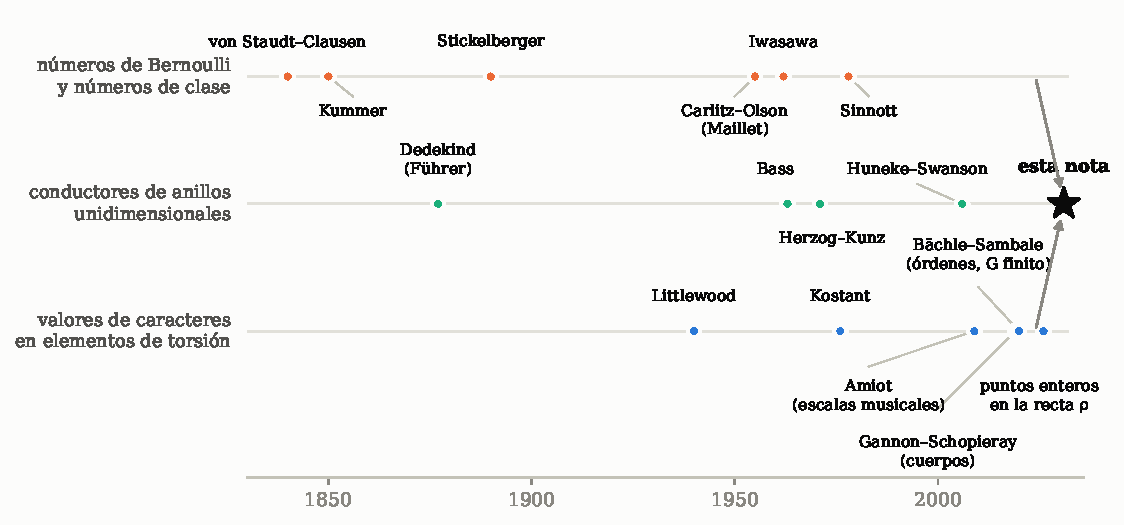
\includegraphics[width=\textwidth]{fig_historia_es.pdf}
\caption{Tres líneas de trabajo, y el punto donde esta nota las une. Las fechas son años de publicación.}
\label{fig:historia}
\end{figure}

\noindent\textbf{Números de Bernoulli y números de clase.} Los números $B_k$ entran en la teoría de números con von
Staudt y Clausen, que localizaron sus denominadores, y con Kummer, que ligó la divisibilidad de sus numeradores por
un primo $p$ al número de clase de $\QQ(\zeta_p)$. El elemento de Stickelberger anula el grupo de clases; Iwasawa y
Sinnott calcularon el índice del ideal que genera, que es el número de clase relativo $h^-$ salvo una potencia de
$2$ \cite{Sin78,Was97}. Entre medias, Maillet preguntó por el determinante de la matriz de restos mínimos
$R(rs^{-1})$, y Carlitz y Olson mostraron que es una potencia de $p$ por $h^-$ \cite{CO55}.

\noindent\textbf{Conductores de anillos de dimensión uno.} Para un anillo reducido $A$ de dimensión uno con
normalización finita $\cO$, el conductor $\cf=(A:\cO)$, el \emph{Führer} de Dedekind, mide cuánto le falta a $A$ para
ser normal. Bass recogió, a partir de Apéry, Gorenstein y Samuel, que un anillo de Gorenstein cumple
$\ell(\cO/A)=\ell(A/\cf)$ \cite[Cor.~(6.5)]{Bas63}; Herzog y Kunz, y
después Huneke y Swanson, situaron la desigualdad correspondiente y su caso de igualdad en la teoría del módulo
canónico \cite{HK71,HS06}.

\noindent\textbf{Valores de caracteres en elementos de torsión.} Kostant destacó elementos en los que todo carácter
de un grupo simple toma uno de los valores $0,\pm1$ \cite[Teor.~3.1]{Kostant76}; para $\Sp(2m)$ uno de ellos, el
elemento principal de tipo $\rho$, es $g_{1/(2m+2)}$. Los cuerpos generados por valores de caracteres se entienden en el marco modular \cite{GS19}, y
para grupos finitos Bächle y Sambale estudiaron los \emph{órdenes} $\ZZ[\chi(g):\chi\in\mathrm{Irr}(G)]$
\cite{BS20}. Para $\Sp(2m)$ a lo largo de la línea $g_{1/q}$, los puntos en los que todo carácter es entero se
clasificaron en \cite{Mar26}, donde se dibuja un mapa de la historia anterior de esa pregunta. Por último, desde la
teoría musical: qué intervalos generan una escala dada en $\ZZ/c$ lo resolvió Amiot \cite{Ami09}, y ese es
exactamente el lema combinatorio que necesita esta nota.

% ==============================================================================================
\section{¿Cuándo es el anillo simplemente \texorpdfstring{$\ZZ$}{Z}?}\label{sec:set}

\pregunta{Antes de preguntar qué falta, conviene saber cuándo no hay nada que falte.}

\noindent Fijemos $q\ge3$, $1\le m<q/2$, $\xi=\xi_q$, $\eta_j=\xi^j+\xi^{-j}$, y $\cO=\ZZ[\xi+\xi^{-1}]$, el
anillo de enteros de $K=\QQ(\xi)^+$. El anillo de representaciones de $\Sp(2m)$ es $\ZZ[e_1,\dots,e_m]$, con $e_i$
las funciones simétricas elementales de $x_1+x_1^{-1},\dots,x_m+x_m^{-1}$; por tanto
\begin{equation}\label{eq:A}
\marco{A=A_m(q)=\ZZ\bigl[e_1(\eta_1,\dots,\eta_m),\dots,e_m(\eta_1,\dots,\eta_m)\bigr]\subseteq\cO}
\end{equation}
Todo depende de cómo se sitúa el segmento $\{\pm1,\dots,\pm m\}$ módulo un entero $n$. Sea
$N^{(n)}(c)=\#\{1\le j\le m: j\equiv\pm c\pmod n\}$ sobre las clases $c\in(\ZZ/n)/\pm1$.

\begin{lemma}[segmentos]\label{lem:seg}
Sea $n\ge3$ y sea $a$ una unidad módulo $n$ con $a\not\equiv\pm1$. Entonces $N^{(n)}$ es estable por $c\mapsto ac$
si y solo si $n$ divide a $h$, $h+1$ o $h+2$; en ese caso es estable por toda unidad.
\end{lemma}

\begin{proof}
Escribamos $m=kn+r$ con $0\le r<n$. Los periodos completos aportan un multiconjunto invariante por las unidades, así
que la estabilidad es la del segmento $\{\pm1,\dots,\pm s\}$ con $s=r$ si $r\le n/2$ y $s=n-1-r$ en otro caso. El
conjunto $[-s,s]\subseteq\ZZ/n$ es una escala generada por $1$; si $a[-s,s]=[-s,s]$ también está generada por $a$, y
por \cite{Ami09}, Teorema~1, un generador coprimo distinto de $\pm1$ obliga a la escala a tener $1$, $n-1$ o $n$
elementos. Esos son $r\in\{0,n-1\}$, $r=(n-1)/2$ para $n$ impar, y $r\in\{n/2-1,n/2\}$ para $n$ par; es decir,
$n\mid h$, $n\mid h+2$ o $n\mid h+1$. Esos segmentos son estables por toda unidad. La misma clasificación, con otra
demostración, está en \cite{Mar26}, Teorema~5.1.
\end{proof}

\noindent La lectura musical es literal. En $\ZZ/12$ la escala diatónica $\{0,2,4,5,7,9,11\}$ es una sucesión de siete
quintas consecutivas, la escala que apila la afinación pitagórica: un segmento para el generador $7$. Tiene siete
notas, ni $1$, ni $11$, ni $12$, así que por el teorema de Amiot ningún generador distinto de $\pm7$ la dispone como
segmento. En el lema los papeles se invierten: el segmento $\{\pm1,\dots,\pm m\}$ lo dispone $1$, y la pregunta es
qué otros generadores admite. La respuesta la gobierna $h=2m$, el número de Coxeter del tipo $C_m$, es decir, el
orden del producto de las reflexiones simples de su grupo de Weyl.

\begin{table}[htbp]
\centering\small
\rowcolors{2}{filaclara}{white}
\begin{tabular}{llll}
\toprule
familia & $m \bmod n$ & el segmento $\{\pm1,\dots,\pm m\}$ módulo $n$ & ejemplo ($m=6$) \\
\midrule
$n\mid h$ & $0$ o $n/2$ & periodos completos ($+$ la clase $n/2$) & $n=4,12$ \\
$n\mid h+1$ & $(n-1)/2$ & cada clase no nula, una vez más & $n=13$ \\
$n\mid h+2$ & $n-1$ o $n/2-1$ & periodos completos menos $\{0\}$ (y $\{n/2\}$) & $n=7,14$ \\
\bottomrule
\end{tabular}
\caption{Las tres familias estables. $h=2m$ es el número de Coxeter del tipo $C_m$.}
\label{tab:familias}
\end{table}

\begin{proposition}[$A=\ZZ$]\label{prop:AZ}
$A=\ZZ$ si y solo si $q\in\{2m+1,2m+2\}$ o $(q,m)=(6,1)$. En otro caso $A$ es un orden de rango $\varphi(q)/2$
en $K$.
\end{proposition}

\begin{proof}
El cuerpo de fracciones de $A$ es el cuerpo fijo del estabilizador de $N^{(q)}$ en
$\mathrm{Gal}(K/\QQ)=(\ZZ/q)^\times/\pm1$. Para $q\notin\{3,4,6\}$ el Lema~\ref{lem:seg} hace ese estabilizador
trivial o total, y con $2m<q$ es total exactamente para $q\in\{2m+1,2m+2\}$. Para
$q\in\{3,4,6\}$, $\cO=\ZZ$; con $2m<q$ esto da $m=1$ para $q=3,4$ y $m\in\{1,2\}$ para $q=6$.
\end{proof}

\noindent Esto no es nuevo. Para $m\ge2$ es la parte $2m<q$ de \cite{Mar26}, Teorema~5.1, cuyo enunciado contiene
además una familia esporádica $q=6$, $m\equiv1\pmod3$, fuera del rango $2m<q$ de aquí; el caso $(6,1)$ es su sombra
con $m=1$. En el lenguaje de los elementos racionales dice que $g_{1/q}$ es conjugado de todas sus potencias primas
con $q$ exactamente en estos puntos, y para $q=2m+2$ el elemento es uno de los de Kostant \cite[Teor.~3.1]{Kostant76}. A partir
de ahora $A\neq\ZZ$ y $\cf=(A:\cO)$.

\begin{lemma}[estabilidad de Galois]\label{lem:galois}
Supongamos $A\ne\ZZ$. El orden $A$ y su conductor $\cf$ son estables por $\mathrm{Gal}(K/\QQ)$. Por tanto, para cada primo $p$, todos los
primos de $\cO$ sobre $p$ aparecen en $\cf$ con el mismo exponente $e_p\ge0$: $\cf\,\cO_p=\rad_p^{\,e_p}$, donde
$\rad_p$ es el radical de $\cO_p=\cO\otimes\ZZ_p$.
\end{lemma}

\begin{proof}
Sea $C_u\in\ZZ[X]$ el polinomio de Chebyshev, reescalado de modo que $C_u(2\cos\theta)=2\cos u\theta$; equivalentemente
$C_u(t+t^{-1})=t^u+t^{-u}$, con $C_0=2$, $C_1=X$, $C_{u+1}=XC_u-C_{u-1}$. Para $\sigma_u(\xi)=\xi^u$ se tiene $\sigma_u(\eta_j)=C_u(\eta_j)$, luego
$\sigma_u(e_k(\eta_1,\dots,\eta_m))=e_k(C_u(\eta_1),\dots,C_u(\eta_m))$, un polinomio simétrico con coeficientes
enteros en $\eta_1,\dots,\eta_m$, y por tanto un elemento de $A$. Así $\sigma_u(A)\subseteq A$ para todo $u$, y la
igualdad se sigue aplicando $\sigma_u^{-1}$. Entonces $\sigma_u(\cf)=(\sigma_u(A):\sigma_u(\cO))=\cf$, y los primos
sobre $p$ forman una sola órbita de Galois.
\end{proof}

\frontera{Los puntos enteros $q\mid h,h+1,h+2$ son del tipo $C$. Para otro grupo simple simplemente conexo, ¿en qué órdenes $q$ es $\exp(2\pi i\rho^\vee/q)$ conjugado a todas sus potencias primas con $q$, y pueden leerse esos $q$ en los números regulares de su grupo de Weyl?}

% ==============================================================================================
\section{¿Qué primos dividen al índice?}\label{sec:sop}

\pregunta{El anillo $A$ tiene índice finito en $\cO$. ¿Siguen algún patrón los primos de ese índice?}

\noindent Para un primo $p$ escribamos $q=p^vq'$ con $p\nmid q'$, $E=\varphi(p^v)$, y sea $f$ el orden de
$p$ en $(\ZZ/q')^\times/\pm1$, el grado residual de $p$ en $K$. Definimos, para $c\in\ZZ/q'$,
\begin{equation}\label{eq:S}
\marco{S(c)=\sum_{\substack{1\le j\le m\\ j\equiv c\ (q')}} j\;-\sum_{\substack{1\le j\le m\\ j\equiv -c\ (q')}} j}
\end{equation}
una función impar en $\ZZ/q'$: el primer momento del segmento, clase a clase.

\begin{keybox}
\begin{theorem}[soporte del conductor]\label{thm:sop}
Supongamos $A\ne\ZZ$.
\begin{enumerate}
\item[(a)] Si $p\nmid q$, entonces $p\nmid[\cO:A]$.
\item[(b)] Sean $p\mid q$ y $q'\ge3$. Entonces $p\mid[\cO:A]$ si y solo si falla al menos una de las siguientes:
 \emph{(i)} el estabilizador de $N^{(q')}$ en $(\ZZ/q')^\times/\pm1$ es trivial;
 \emph{(ii)} $E=1$, o $S(c)\not\equiv0\pmod p$ para algún $c$ con $2c\not\equiv0\pmod{q'}$.
\item[(c)] Si $p\mid q$ y $q'\notin\{1,2,3,4,6\}$, entonces
 \[ p\mid[\cO:A]\iff q'\mid h,\ \ q'\mid h+1\ \ \text{o}\ \ q'\mid h+2 . \]
\end{enumerate}
\end{theorem}
\end{keybox}

\noindent Leída a través de un primo $\mathfrak P$ de $\ZZ[\xi]$ sobre $p$, la parte~(c) dice: la reducción mata la
parte de $g$ de orden potencia de $p$ y deja su parte prima con $p$, de orden $q'$; y para $q'\notin\{3,4,6\}$, $p$
divide al índice exactamente cuando esa parte está en una de las tres familias $q'\mid h,h+1,h+2$ de puntos enteros
(\cite{Mar26}, Teorema~5.1; la Proposición~\ref{prop:AZ} es su parte con $2m<q'$).
Para el ejemplo guía $A_3(35)$: en $p=7$ la parte $q'=5$ no divide a ninguno de $h,h+1,h+2=6,7,8$, luego
$7\nmid[\cO:A]$; en $p=5$, $q'=7=h+1$, luego $5\mid[\cO:A]$.
La Figura~\ref{fig:paisaje} muestra el índice sobre el plano $(q,m)$, separado por primos y coloreado por familia.

\begin{proof}
Como $[\cO:A]$ es finito, $p\nmid[\cO:A]$ si y solo si $A+p\cO=\cO$, es decir, la imagen de $A$ en $\cO/p\cO$ es
todo.

(a) Para $p\nmid q$, $\cO/p\cO$ es étale y sus puntos en $\overline{\FF}_p$ son las reducciones de
$\xi\mapsto\xi^u$, $u\in(\ZZ/q)^\times/\pm1$. En el punto $u$ las $e_i$ son las funciones simétricas elementales
de $u\cdot N^{(q)}$, y multiconjuntos distintos dan puntos distintos porque $c\mapsto\omega^c+\omega^{-c}$ es
inyectiva sobre las clases para una raíz primitiva $\omega$ de orden $q$ en característica $p$. Así $A$ genera
$\cO/p\cO$ si y solo si el estabilizador de $N^{(q)}$ es trivial, si y solo si $A\ne\ZZ$ (Lema~\ref{lem:seg},
Proposición~\ref{prop:AZ}). Para los órdenes generados por todos los caracteres irreducibles de un grupo finito $G$,
el hecho análogo, que los primos del índice dividen a $|G|$, es \cite{BS20}, Proposición~6; no se aplica a $A$
directamente, porque $A$ está generado solo por caracteres de $\Sp(2m)$.

(b) En $\ZZ_p[\xi]$ escribamos $\xi=\omega(1+\pi)$ con $\omega$ de orden $q'$ y $1+\pi$ de orden $p^v$; entonces
$\ZZ[\xi]/p=\FF_p[\omega][\pi]/(\pi^E)$. Como $q'\ge3$, la conjugación compleja no está en el grupo de inercia, así que
$\cO/p\cO\cong\prod_{P\mid p}\FF_{p^f}[z]/(z^E)$ con $z=\eta_1-(\omega+\omega^{-1})\equiv(\omega-\omega^{-1})\pi$.
Sean $\rad$ el radical y $\bar R=\cO/\rad$ el anillo residual. Si $E=1$, entonces $\cO/p\cO=\bar R$ y solo importa
(i): el argumento de (a) vale con $q'$ en lugar de $q$. Supongamos $E\ge2$, y sea $B_2$ la imagen de $A$ en
$\Lambda_2=\cO/(p,\rad^2)=\bar R[z]/(z^2)$. Si $B_2=\Lambda_2$, la imagen de $A$ en $\cO/p\cO$ contiene $\bar R$ (a
través de $x\mapsto x^{p^N}$, que mata $z$) y un generador de $\rad/\rad^2$, luego todo; el recíproco es claro.
Módulo $\rad^2$, $\eta_j\equiv\gamma_j+jU_jz$ con $\gamma_j=\omega^j+\omega^{-j}$ y
$U_j=(\omega^j-\omega^{-j})/(\omega-\omega^{-1})$, así que $\prod_j(T-\eta_j)\equiv F(T)-zG(T)$ con
$F=\prod_j(T-\gamma_j)$ y
\begin{equation}\label{eq:G}
\marco{G=F\sum_j\frac{jU_j}{T-\gamma_j}=F\sum_{c}\frac{S(c)\,U_c}{T-\gamma_c},}
\end{equation}
donde la segunda suma recorre las clases con $N^{(q')}(c)\ge1$. Los coeficientes de $F$ generan $\bar R$ si y solo si
el estabilizador de $N^{(q')}$ es trivial, como en (a). En ese caso $\bar R\subseteq B_2$, y la parte en $z$ de $B_2$
es el $\bar R$-submódulo generado por los coeficientes de $G$, que es todo $z\bar R$ si y solo si $G$ no se anula en
ningún cuerpo residual. Las funciones $U_cF/(T-\gamma_c)$ con $2c\not\equiv0$ y $N^{(q')}(c)\ge1$ son linealmente
independientes, así que esto ocurre si y solo si $S(c)\not\equiv0\pmod p$ para algún tal $c$.

(c) Por el Lema~\ref{lem:seg}, (i) falla si y solo si $q'\mid h,h+1,h+2$. Cuando (i) se cumple, $m=kq'+r$ con $r$
fuera de la lista de ese lema, y contando se obtiene, para $1\le c\le q'-1$,
\[
S(c)=\begin{cases}(2k+1)c & c\le r<q'-c,\\ -(2k+1)(q'-c) & q'-c\le r<c,\\ (k+1)(2c-q') & q'-c\le r\ \text{y}\ c\le r,\\
k(2c-q') & r<c\ \text{y}\ r<q'-c.\end{cases}
\]
Escribamos $n=q'$. Como $r\notin\{0,n-1\}$, el resto $c=1$ cae en el primer caso y $S(1)=2k+1$. Si $r<n/2$
(luego $r<(n-1)/2$ para $n$ impar y $r<n/2-1$ para $n$ par), tomemos $c=(n-1)/2$ para $n$ impar, que da $S(c)=-k$,
o $c=n/2-1$ para $n$ par, que da $S(c)=-2k$. Si $r>n/2$,
tomemos $c=(n+1)/2$ o $c=n/2+1$, que dan $S(c)=k+1$ o $2(k+1)$. En todos los casos $p$ no puede dividir a la vez a
$S(1)=2k+1$ y a $S(c)$, pues $\gcd(2k+1,k)=\gcd(2k+1,k+1)=1$. Así (ii) se cumple siempre que se cumpla (i), también
para $p=2$.
\end{proof}

\begin{figure}[!htbp]
\centering
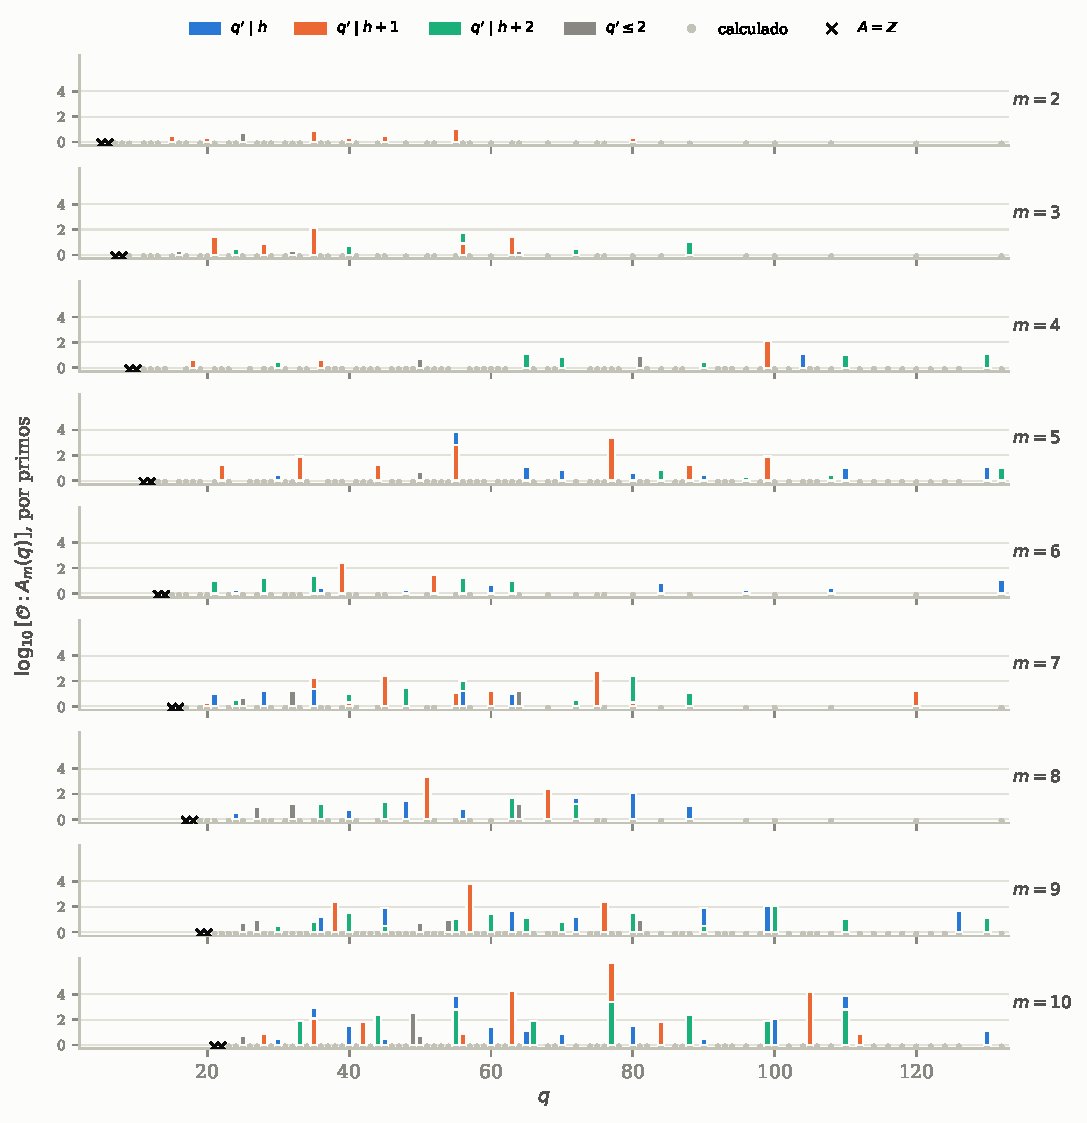
\includegraphics[width=\textwidth]{fig_paisaje2d_es.pdf}
\caption{El índice $[\cO:A_m(q)]$ para $2\le m\le10$ y $q\le132$ ($558$ órdenes con cálculo de retículo, $156$
de ellos con índice $>1$), un panel por cada $m$. Cada barra se apila por los primos $p$ del índice, cada tramo de
altura $v_p\cdot\log_{10}p$ y coloreado por la familia de $q'=q/p^{v}$; los tramos grises son primos con $q'\le2$,
fuera de los teoremas. Los puntos marcan los $q$ calculados (sin barra: índice $1$); las cruces marcan $A=\ZZ$. Todo
tramo coloreado está sobre un par con $q'\mid h,h+1,h+2$.}
\label{fig:paisaje}
\end{figure}

\frontera{El Teorema~\ref{thm:sop}(b) tiene dos cláusulas: una étale, sobre el estabilizador de Galois de la parte de $g$ prima con $p$, y otra tangente, sobre el primer momento. Para un elemento de torsión de cualquier grupo simplemente conexo, ¿sigue siendo $p\mid[\cO:\ZZ[\chi(g)]]$ el fallo de una de las dos, con la diferencial de los caracteres fundamentales en el papel de $S$?}

% ==============================================================================================
\section{¿Cómo es el defecto en un primo?}\label{sec:loc}

\pregunta{Sabiendo que $p$ divide al índice, uno querría ver el conductor en $p$: cuántos ideales maximales, qué
cuerpos residuales, a qué profundidad.}

\noindent Supongamos $p\mid q$, $q'\notin\{1,2,3,4,6\}$, $E\ge2$, y $q'\mid h,h+1,h+2$, de modo que $p\mid[\cO:A]$ y
$N^{(q')}$ es estable por toda unidad. Sean $\rad$ el radical de $\cO_p=\cO\otimes\ZZ_p$, $A_p=A\otimes\ZZ_p$,
$d=\varphi(q')/2=\dim_{\FF_p}\bar R$, y sea $\gr_i(A)$ la imagen de $A_p\cap\rad^i$ en
$\rad^i/\rad^{i+1}\cong\bar R$. Pongamos $W_i=\dim_{\FF_p}\gr_i(A)$, de modo que $W_0=1$ y $W_i\le d$; por el
Lema~\ref{lem:galois}, $\cf\,\cO_p=\rad^{e}$ para un único exponente $e=e_p$.

\begin{keybox}
\begin{theorem}[estructura local]\label{thm:loc}
Bajo estas hipótesis:
\begin{enumerate}
\item[(a)] la imagen de $A$ en $\bar R$ es $\FF_p$; así que $A$ tiene exactamente un ideal maximal sobre $p$, que
 contiene a $\cf$, y su cuerpo residual es $\FF_p$;
\item[(b)] $W_1=\dim_{\FF_p}\FF_p[(\ZZ/q')^\times]\cdot S$, donde $(u\cdot S)(c)=S(u^{-1}c)$;
\item[(c)] $e=1$ si y solo si $W_1=d$;
\item[(d)] $v_p([\cO:A])=\sum_{i=0}^{e-1}(d-W_i)$ y $v_p([A:\cf])=\sum_{i=0}^{e-1}W_i$; en particular, si $e=2$,
 entonces $v_p([A:\cf])=1+W_1$ y $v_p([\cO:A])=2d-1-W_1$.
\end{enumerate}
\end{theorem}
\end{keybox}

\begin{proof}
(a) La estabilidad hace $F\in\FF_p[T]$: las $e_i$ se reducen a las mismas constantes de $\FF_p$ en cada cuerpo
residual. Por el Teorema~\ref{thm:sop}, $p\mid[\cO:A]$, así que ese ideal contiene a $\cf$.

(b) Todo elemento de $A$ es $\Phi(e)$ con $\Phi\in\ZZ[X]$; módulo $\rad^2$,
$\Phi(e)\equiv\Phi(F)+z\sum_i(\partial_i\Phi)(F)G_i$ con $\Phi(F)\in\FF_p$, y $p\in\rad^2$. Por tanto $\gr_1(A)$ es
el $\FF_p$-subespacio $V$ generado por los coeficientes $G_i$. Como $\bar R$ es étale,
$\bar R\otimes_{\FF_p}\overline{\FF}_p\cong\overline{\FF}_p^{\,d}$, con coordenadas las $d$ inmersiones
$\sigma_u\colon\omega+\omega^{-1}\mapsto\omega_0^u+\omega_0^{-u}$, $u\in(\ZZ/q')^\times/\pm1$, para un
$\omega_0\in\overline{\FF}_p$ fijo de orden $q'$. La extensión de escalares es inyectiva sobre los
$\FF_p$-subespacios, así que $\dim_{\FF_p}V$ es el rango sobre $\overline{\FF}_p$ de la matriz cuya fila $u$ lista los
coeficientes de $\sigma_u(G)$. Multiplicar la fila $u$ por la unidad $U_u$ no cambia ese rango. De
$\sigma_u(\gamma_c)=\gamma_{uc}$, $\sigma_u(U_c)=U_{uc}/U_u$ y la estabilidad de $F$,
\begin{equation}\label{eq:rango}
\marco{U_u\,\sigma_u(G)=\sum_c S(u^{-1}c)\;U_c\,\frac{F(T)}{T-\gamma_c},}
\end{equation}
y las funciones $U_cF/(T-\gamma_c)$, sobre las clases $c$ con $2c\not\equiv0\pmod{q'}$ (para las demás $U_c=0$), son
linealmente independientes sobre $\overline{\FF}_p$ y no dependen de $u$.
Así el rango es el de $[S(u^{-1}c)]_{u,c}$, una matriz con entradas en $\FF_p$, cuyo rango sobre
$\overline{\FF}_p$ es igual a su rango sobre $\FF_p$, que es $\dim_{\FF_p}\FF_p[(\ZZ/q')^\times]\cdot S$.

(c) Si $\gr_1(A)=\gr_1(\cO)$, entonces $\gr_i(A)\supseteq\gr_1(A)^i=\gr_i(\cO)$ para todo $i\ge1$, porque $\gr(\cO_p)$ es
un anillo de polinomios sobre $\bar R$; así el subretículo cerrado $A_p\cap\rad$ tiene el graduado de $\rad$ y
coincide con él. El recíproco es claro.

(d) Filtremos $\cO_p$ y $A_p$ por los $\rad^i$. Para $i\ge e$, $A_p\cap\rad^i=\rad^i$, así que solo contribuyen las
capas $i<e$: $\cO_p/A_p$ tiene una filtración con cocientes de dimensión $d-W_i$, y $A_p/\cf\cO_p=A_p/\rad^e$
una con cocientes de dimensión $W_i$.
\end{proof}

\noindent\textbf{El ejemplo guía.} Para $A_3(35)$ en $p=5$: $E=4$, $q'=7$, $d=3$, y como $m=3<7$ el primer
momento es simplemente $S(c)=c$ para $c=1,2,3$ (y $S(-c)=-S(c)$). Con filas $u=1,2,3$ y columnas $c=1,2,3$, y
$u^{-1}\equiv1,4,5\pmod 7$,
\[
\bigl[S(u^{-1}c)\bigr]=\begin{pmatrix}1&2&3\\-3&1&-2\\-2&3&1\end{pmatrix},
\]
cuyo determinante es $0$ y cuyo rango es $2$ sobre $\QQ$ y módulo $5$. Así $W_1=2<d=3$ y, por el
Teorema~\ref{thm:loc}(c), el conductor en $5$ no es el radical. Por qué la matriz es singular ya sobre $\ZZ$ se
explica en el \S\ref{sec:clase}.

\noindent Los productos de capas las hacen utilizables en la práctica. Como $\gr(A)$ es un subanillo de
$\gr(\cO_p)$, las capas se multiplican: $\gr_i(A)\cdot\gr_j(A)\subseteq\gr_{i+j}(A)$. Escribamos $\bar R=\prod_{a=1}^{g}k_a$ e
identifiquemos cada capa con $\bar R$ mediante uniformizantes $z_a$ de los factores; por el Lema~\ref{lem:galois} el grupo
$\mathrm{Gal}(K/\QQ)$ permuta los factores transitivamente y conserva $A_p\cap\rad^i$, y actúa sobre cada capa por una
permutación de los factores, semilineal en cada factor y torcida por unidades.

\begin{proposition}[crecimiento de las capas]\label{prop:cert}
Bajo las hipótesis del Teorema~\ref{thm:loc}, sea $s\ge1$ con $W_s>0$. Entonces $W_{i+s}\ge W_i$ para todo $i\ge0$. Por tanto:
\begin{enumerate}
\item[(a)] si $W_a=W_{a+1}=\dots=W_{a+s-1}=d$ para algún $a$, entonces $\rad^a\subseteq A_p$ y $e\le a$; esto vale con
 $s=E$, porque $p\in A_p\cap\rad^E$ tiene imagen no nula en $\gr_E(A)$;
\item[(b)] si $W_1>0$, entonces $e$ es el menor $i$ con $W_i=d$.
\end{enumerate}
\end{proposition}

\begin{proof}
La imagen $V_s=\gr_s(A)\subseteq\bar R$ es no nula y estable por la acción torcida, así que su proyección sobre
cada factor $k_a$ es no nula. Si $v_1,\dots,v_r$ es una base de $V_s$, el elemento $v=\sum_k T^{k-1}v_k$ de
$\bar R\otimes_{\FF_p}\FF_p(T)=\prod_ak_a(T)$ tiene todas sus componentes no nulas, luego es una unidad, y la
multiplicación por $v$ sumerge $\gr_i(A)\otimes\FF_p(T)$ en $\gr_{i+s}(A)\otimes\FF_p(T)$; la extensión de escalares
conserva las dimensiones, así que $W_i\le W_{i+s}$. (a) Por inducción toda capa a partir de $a$ está llena, y
$A_p\cap\rad^a$, un subretículo cerrado con el graduado de $\rad^a$, es igual a $\rad^a$. Como el conductor conmuta
con $\otimes\ZZ_p$ y $\rad^a$ es un ideal de $\cO_p$, $\rad^a\subseteq A_p$ da $\rad^a\subseteq\cf\cO_p$, es decir,
$e\le a$. (b) Tomemos $s=1$ en (a): una capa llena $k$ da $e\le k$; recíprocamente, $\rad^e\subseteq A_p$ hace $W_e=d$.
\end{proof}

\noindent Como $W_0=1<d$, entre las capas $0\le i<E$ hay a lo sumo $E-1$ llenas, así que un cálculo limitado a $i<E$
no puede usar (a) con $s=E$; (b) solo necesita $W_1>0$ y una capa llena. Se pueden usar varios pasos a la vez.

\begin{corollary}[certificación por semigrupos]\label{cor:semigrupo}
Bajo las hipótesis del Teorema~\ref{thm:loc}, sea $\Sigma$ el monoide aditivo (que contiene a $0$) generado por los grados $s\ge1$
con $W_s>0$. Si $W_a=d$, entonces $W_{a+\sigma}=d$ para todo $\sigma\in\Sigma$. En particular, si todo grado $i\ge a$
es de la forma $a'+\sigma$ con $W_{a'}=d$ y $\sigma\in\Sigma$, entonces $e\le a$.
\end{corollary}

\begin{proof}
Apliquemos la Proposición~\ref{prop:cert} una vez por cada generador en una descomposición de $\sigma$; la última
afirmación se sigue como en la Proposición~\ref{prop:cert}(a).
\end{proof}

\noindent Un segundo argumento de productos acota las capas por arriba.

\begin{proposition}[capas complementarias]\label{prop:mono}
Bajo las hipótesis del Teorema~\ref{thm:loc}, si $W_{i+j}<d$ entonces $W_i+W_j\le d$. En particular:
\begin{enumerate}
\item[(a)] $W_i+W_{e-1-i}\le d$ para $0\le i<e$, luego $2\sum_{i<e}W_i\le ed$;
\item[(b)] si $d/2<W_1<d$, entonces $e=2$.
\end{enumerate}
Para $i+j=e-1$ la desigualdad es el caso diagonal de \cite{CDK94}, Corolario~(3.7).
\end{proposition}

\begin{proof}
Extendamos escalares a $\overline{\FF}_p$, de modo que $\bar R\otimes\overline{\FF}_p=\overline{\FF}_p^{\,d}$ con
coordenadas indexadas por los puntos geométricos, que $\mathrm{Gal}(K/\QQ)$ permuta transitivamente, y los productos
de capas se calculan coordenada a coordenada. Si $V_{i+j}=\gr_{i+j}(A)\otimes\overline{\FF}_p$ es un subespacio propio,
su anulador en el dual es no nulo y estable por la acción torcida; una combinación lineal genérica de los trasladados
de un funcional anulador no nulo es un funcional $\lambda(x)=\sum_a\lambda_ax_a$ del anulador con todos los
$\lambda_a\neq0$. La forma $B_\lambda(x,y)=\lambda(xy)$ es no degenerada, y $B_\lambda(V_i,V_j)\subseteq
\lambda(V_{i+j})=0$, así que $W_i+W_j\le d$. (a) $W_{e-1}<d$: si no, toda capa a partir de $e-1$ estaría llena y
$\rad^{e-1}\subseteq A_p$, como en la demostración de la Proposición~\ref{prop:cert}(a). Sumando sobre $i$ se obtiene la
segunda desigualdad. (b) $2W_1>d$ obliga a $W_2=d$; por la Proposición~\ref{prop:cert}(b), $e\le2$, y $e\ge2$ por el
Teorema~\ref{thm:loc}(c).
\end{proof}

\begin{proposition}[un solo primo sobre $p$]\label{prop:unprimo}
Bajo las hipótesis del Teorema~\ref{thm:loc}, supongamos que $p$ tiene un solo primo sobre él en $K$, de grado
residual primo $f=d\ge3$, y que $2\le W_1<d$. Entonces $2\le e\le d-1$. En particular $e=2$ cuando $d=3$.
\end{proposition}

\begin{proof}
$\bar R=\FF_{p^d}$. Elijamos $a,b\in\gr_1(A)$ linealmente independientes sobre $\FF_p$ y pongamos $t=b/a\notin\FF_p$;
como $d$ es primo, $t$ genera $\FF_{p^d}$, así que $1,t,\dots,t^{d-1}$ es una base. Los productos de $k$ elementos de
$\gr_1(A)$ están en $\gr_k(A)$ e incluyen $a^k,a^{k-1}b,\dots,b^k=a^k(1,t,\dots,t^k)$, que generan $\bar R$ en cuanto
$k\ge d-1$. Así toda capa $k\ge d-1$ está llena, luego $\rad^{d-1}\subseteq A_p$ (como en la demostración de la
Proposición~\ref{prop:cert}); y $e\ge2$ por el Teorema~\ref{thm:loc}(c).
\end{proof}

\begin{proposition}[el criterio de Gorenstein, en capas]\label{prop:gor}
Bajo las hipótesis del Teorema~\ref{thm:loc}, $A_p$ es de Gorenstein si y solo si $\ell(\cO_p/A_p)=\ell(A_p/\cf\cO_p)$,
es decir, si y solo si $2\sum_{i<e}W_i=ed$, es decir, si y solo si
\[
W_i+W_{e-1-i}=d\qquad\text{para todo }0\le i<e .
\]
Cuando $e=2$ esto se lee $W_1=d-1$.
\end{proposition}

\begin{proof}
Que un anillo de Gorenstein se caracteriza por la igualdad de longitudes es clásico: Bass demuestra una dirección
\cite[Cor.~(6.5)]{Bas63} y recoge allí el recíproco a partir de Serre y Grothendieck; véanse también \cite{HK71} y
\cite{HS06}, Corolario~12.2.4. La forma simétrica es el caso diagonal del criterio de Campillo, Delgado y
Kiyek \cite{CDK94}, (3.6)--(3.7), enunciado para anillos locales de Cohen--Macaulay de dimensión uno analíticamente
reducidos con extensiones residuales arbitrarias; aquí damos un argumento directo para el caso que nos ocupa. Por el
Teorema~\ref{thm:loc}(a), $R=A_p$ es local con cuerpo residual $\FF_p$; es finito sobre $\ZZ_p$, luego completo,
reducido de dimensión uno, con normalización finita $\cO_p$ y conductor $\cf\cO_p=\cf\otimes\ZZ_p$ (cambio de base
plano). Todo factor de composición de un $R$-módulo finito es $\FF_p$, así que su longitud es el $\log_p$ de su
cardinal; las capas están anuladas por $p$, y en ellas las longitudes son $\FF_p$-dimensiones. Así las dos primeras
formas de la condición coinciden por el Teorema~\ref{thm:loc}(d), y la tercera es el caso de igualdad de la
Proposición~\ref{prop:mono}(a). Si $R$ es de Gorenstein, la igualdad vale por
\cite[Cor.~(6.5)]{Bas63}, o por \cite{HS06}, Teorema~12.2.2, que no hace ninguna hipótesis sobre el cuerpo residual. El
recíproco es \cite{HS06}, Corolario~12.2.4, para un anillo local de dimensión uno analíticamente no ramificado, con
cuerpo residual infinito y un módulo canónico contenido en el anillo; llegamos a él a través de $S=R[T]_{\mathfrak mR[T]}$.
La aplicación $R\to S$ es plana y local, con fibra cerrada $\FF_p(T)$. El anillo $S$ es una localización de un álgebra
finitamente generada sobre un anillo local completo, luego excelente; por ser excelente y reducido, es analíticamente
no ramificado. Su normalización es la localización correspondiente de $\cO_p[T]$, que es normal y finito sobre $R[T]$.
El conductor es $\mathrm{Ann}_R(\cO_p/R)$, y los anuladores de módulos finitamente generados conmutan con el cambio de
base plano, así que el conductor de $S$ es $\cf S$. Las longitudes se conservan, porque cada factor de composición
$\FF_p$ se convierte en $\FF_p(T)$. Por último, $S$ es de Cohen--Macaulay (reducido de dimensión uno), cociente de un
anillo local regular y genéricamente de Gorenstein, así que tiene un módulo canónico
isomorfo a un ideal \cite[Teor.~3.3.6, Prop.~3.3.18(b)]{BH98}. Por tanto la igualdad para $R$ da la igualdad para $S$, luego $S$ es de
Gorenstein por \cite{HS06}, Corolario~12.2.4, y también lo es $R$, porque un homomorfismo local plano de anillos
locales noetherianos con destino de Gorenstein tiene origen de Gorenstein \cite[Tag~0BJL]{Stacks}.
\end{proof}

\begin{figure}[htbp]
\centering
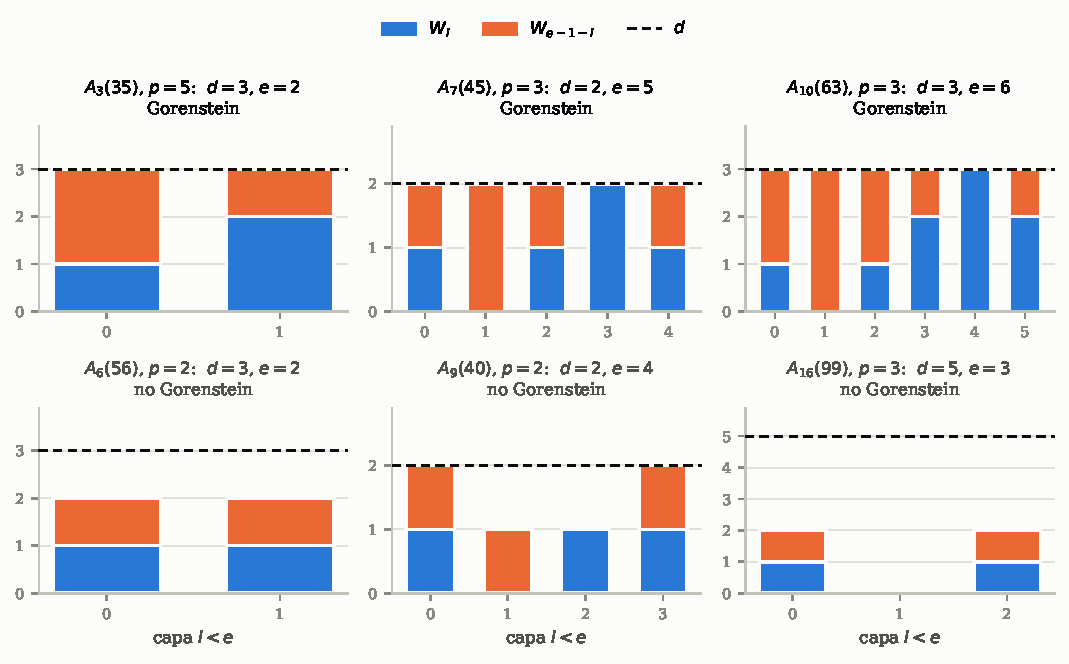
\includegraphics[width=\textwidth]{fig_simetria_es.pdf}
\caption{La Proposición~\ref{prop:gor} en seis cálculos de retículo. La columna $i<e$ apila $W_i$ y su reflejo
$W_{e-1-i}$; por la Proposición~\ref{prop:mono} ninguna columna pasa de $d$, y el anillo local es de Gorenstein
exactamente cuando todas las columnas llegan a $d$. Arriba: $A_3(35)$, $A_7(45)$, $A_{10}(63)$; abajo: $A_6(56)$,
$A_9(40)$, $A_{16}(99)$. En cada panel la simetría coincide con $v_p([\cO:A])=v_p([A:\cf])$ calculado sobre el
retículo.}
\label{fig:simetria}
\end{figure}

\noindent La propiedad de Gorenstein es el caso $\operatorname{type}(A_p)=1$ de un invariante más fino. Cuando el
conductor es el cuadrado del radical, el tipo se lee en la primera capa y en su anillo de multiplicadores.

\begin{proposition}[el tipo cuando $e=2$]\label{prop:tipo}
Bajo las hipótesis del Teorema~\ref{thm:loc}, supongamos $e=2$. Sean $V=\gr_1(A)\subseteq\bar R$ y
$\kappa=\dim_{\FF_p}\{a\in\bar R:\ aV\subseteq V\}$. Entonces el tipo de Cohen--Macaulay de $A_p$ es
\[
\marco{\operatorname{type}(A_p)=d-W_1+\kappa-1,}
\]
$d-W_1\ge\kappa$, y $A_p$ es casi Gorenstein (almost Gorenstein), $\ell(\cO_p/A_p)=\ell(A_p/\cf\cO_p)+\operatorname{type}(A_p)-1$,
si y solo si $d-W_1=\kappa$.
\end{proposition}

\begin{proof}
Sea $\mathfrak m=A_p\cap\rad$, el ideal maximal de $A_p$. Como $A_p\ne\cO_p$, $\mathfrak m$ no es invertible
\cite[Lemma~2.14]{Mars24}, y por \cite{Mars24}, Proposición~3.5,
$\operatorname{type}(A_p)+1=\dim_{\FF_p}(\mathfrak m:\mathfrak m)/\mathfrak m$, y $(\mathfrak m:\mathfrak m)$, un anillo
finito sobre $A_p$, está contenido en $\cO_p$. Como $e=2$, $\rad^2\subseteq A_p$ y $\mathfrak m/\rad^2$ es la capa $V$.
Para $x\in\cO_p$, $x\rad^2\subseteq\rad^2$, y $x\mathfrak m\subseteq\mathfrak m$ si y solo si el residuo $\bar x$
cumple $\bar xV\subseteq V$. Por tanto $(\mathfrak m:\mathfrak m)=\{x\in\cO_p:\bar xV\subseteq V\}$ contiene a $\rad$, y
$\dim(\mathfrak m:\mathfrak m)/\mathfrak m=\kappa+(d-W_1)$. Por el Teorema~\ref{thm:loc}(d), $\ell(\cO_p/A_p)=2d-1-W_1$ y
$\ell(A_p/\cf\cO_p)=1+W_1$, así que la igualdad de casi Gorenstein se lee $d-W_1=\kappa$. La desigualdad es
\cite{HS06}, Teorema~12.2.3, aplicado a $S=A_p[T]_{\mathfrak mA_p[T]}$ como en la demostración de la
Proposición~\ref{prop:gor}; las longitudes y el tipo no cambian por esa extensión local plana con fibra un cuerpo,
porque $\mathrm{Ext}$ conmuta con el cambio de base plano.
\end{proof}

\noindent La definición de anillo casi Gorenstein es la de Barucci y Fröberg \cite{BF97}, en la forma de longitudes
que usa Marseglia \cite{Mars24}, \S7.2. En los $403$ pares (orden, primo) con $q\le250$ en los que las capas
calculadas certifican $e=2$, el tipo calculado a partir del ideal cociente módulo $\rad^2$ coincide con la fórmula,
incluidos $19$ con $\kappa>1$, $9$ de ellos también mediante un cociente sobre el retículo; lo mismo ocurre en los $63$
pares de retículo con $e=2$ (\emph{medido}, \S\ref{sec:metodo}).

% ==============================================================================================
\section{¿Por qué aparecen números de clase?}\label{sec:clase}

\pregunta{El Teorema~\ref{thm:loc} reduce la primera capa, y con ella el criterio para que el conductor en $p$ sea
el radical, al rango de una sola matriz construida con $S$.
¿Dónde se han visto antes matrices así?}

\noindent Miremos $S$ en las familias de la Tabla~\ref{tab:familias}. Si $m=Nq'$ o $m=Nq'-1$, entonces
$S(c)=N(2c-q')$ para $1\le c\le q'-1$: salvo el factor $2Nq'$, el diente de sierra $B_1(c/q')$, cuyos coeficientes
son los del elemento de Stickelberger. Si $2m+1=Nq'$ con $q'$ impar, entonces $S(c)=N\hat c$, con
$\hat c\in(-q'/2,q'/2)$ el resto con signo: el mismo diente de sierra desplazado medio periodo
(Figura~\ref{fig:sierra}). Para $q'=2r$ par, las dos familias estables restantes de la
Tabla~\ref{tab:familias}, $m=Br$ y $m=Br-1$ con $B$ impar, dan también el diente desplazado de periodo $q'$:
$S(c)=B\,\hat s_{q'}(c)$, donde $\hat s_{q'}(c)=\hat c$ es el resto con signo módulo $q'$ y $\hat s_{q'}(r)=0$.

\noindent Solo aparecen estas dos funciones, y una línea dice por qué. Una suma es su cardinal por su media:
escribiendo $C(c)$ para el número de $j\in[-m,m]$ con $j\equiv c\pmod{q'}$ y $\mu(c)$ para el punto medio de esa
progresión aritmética, $S(c)=C(c)\,\mu(c)$ siempre que no sea vacía. Lo que fija la familia es el punto medio. Para
$m\equiv0,-1\pmod{q'}$ toda clase $c\neq0$ tiene $C(c)=2N$ y $\mu(c)=c-q'/2=s_{q'}(c)/2$; para $2m+1=Nq'$ toda
clase tiene $C(c)=N$ y $\mu(c)=\hat c$; en las familias de medio periodo, $C(c)=B$ y $\mu(c)=\hat c$ fuera de las
dos clases $0$ y $q'/2$ que $c\mapsto-c$ deja fijas, donde $S$ se anula de todos modos. Los dos puntos medios son
el diente de sierra y su desplazado, y la multiplicidad es el cardinal.

\begin{figure}[htbp]
\centering
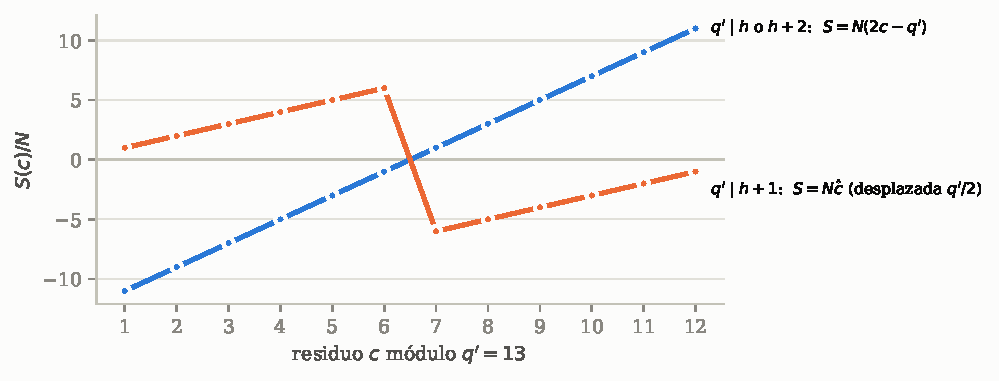
\includegraphics[width=0.78\textwidth]{fig_sierra_es.pdf}
\caption{La función de primer momento $S$ para $q'=13$ en los dos tipos de segmento estable.}
\label{fig:sierra}
\end{figure}

\noindent Para las dos primeras familias la matriz del Teorema~\ref{thm:loc}(b) es, salvo el factor $N$, la
\emph{matriz de momentos}
\[
M_n=\bigl[s_n(u^{-1}c)\bigr],\qquad s_n(0)=0,\quad s_n(c)=2c-n\ (1\le c<n),
\]
con filas $u$ que recorren representantes de $(\ZZ/n)^\times/\pm1$ y columnas que recorren \emph{todos} los restos
$1\le c<n$, unidades o no. Sus menores maximales los gobierna el índice de Sinnott del ideal de Stickelberger.

\noindent Los dos tipos de segmento llevan a dos aritméticas distintas. Las respuestas, enunciadas juntas:

\begin{keybox}
\begin{theorem}[números de clase]\label{thm:hminus}
Sean $p$ impar y $p\mid q$.
\begin{enumerate}
\item[(a)] Si $q'\notin\{1,2,3,4,6\}$, $m\equiv0$ o $-1\pmod{q'}$ y $p\nmid N:=\lceil
 m/q'\rceil$, entonces $d-W_1$ es el número de divisores elementales de $M_{q'}$ divisibles por $p$. Lo mismo vale en
 las familias de medio periodo: para $q'\ge8$ par, $r=q'/2$, $m\equiv r$ o $r-1\pmod{q'}$ y $p\nmid B:=\lceil
 m/r\rceil$. En ambos casos $\cf\,\cO_p=\rad$ si y solo si $p\nmid h^-(\QQ(\zeta_{q'}))$.
\item[(b)] Si $q'\ge5$ es primo y $2m+1=Nq'$ con $p\nmid N(q'-1)$, entonces
 \[W_1=\#\bigl\{\chi\ \text{impar módulo}\ q' : (\overline\chi(2)-1)\,B_{1,\chi}\not\equiv0\pmod{\mathfrak p}\bigr\}\]
 para cualquier primo $\mathfrak p$ sobre $p$ en $\QQ(\mu_{q'-1})$.
\end{enumerate}
\end{theorem}
\end{keybox}

\subsection{El diente de sierra y el ideal de Stickelberger}\label{sec:saw}

\begin{proposition}[el índice de Sinnott, en la matriz de momentos]\label{prop:sinnott}
Sean $n\ge3$, $n\not\equiv2\pmod4$, $d=\varphi(n)/2$, y sea $\Delta_n$ el máximo común divisor de los menores
$d\times d$ de $M_n$. Entonces
\begin{equation}\label{eq:sinnott}
\marco{\Delta_n=2^{a}\,h^-(\QQ(\zeta_n))\,\frac{(2n)^d}{w_n},}
\end{equation}
donde $w_n$ es el número de raíces de la unidad en $\QQ(\zeta_n)$, $a=0$ si $n$ es potencia de un primo y
$a=2^{t-2}-1$ si $n$ tiene $t\ge2$ factores primos. En particular, para un primo impar $p\nmid n$,
$v_p(\Delta_n)=v_p(h^-)$, y el rango de $M_n$ módulo $p$ es $d$ menos el número de divisores elementales de $M_n$
divisibles por $p$.
\end{proposition}

\begin{proof}
Es la fórmula del índice de Sinnott \cite{Sin78,Sin80} leída a través de los generadores de Bernard y Kučera \cite{BK24}.
Sea $G=(\ZZ/n)^\times$ y, para $0<c<n$, $\omega_n(c)=\sum_{u\in G}\bigl(\langle-cu/n\rangle-\tfrac12\bigr)\sigma_u^{-1}$, con
$\langle x\rangle$ la parte fraccionaria. Cambiando $u$ por $u^{-1}$ y usando $\langle-x\rangle-\tfrac12=-(\langle
x\rangle-\tfrac12)$ para $x\notin\ZZ$,
\[
\sum_{u\in G}s_n(u^{-1}c)\,\sigma_u=-2n\,\omega_n(c),
\]
tanto para unidades como para no unidades. Cada $\omega_n(c)$ es impar, así que las columnas de $M_n$ son las
coordenadas de $-2n\,\omega_n(c)$ en la base $\sigma_u-\sigma_{-u}$ de $R^-=\{\alpha\in\ZZ[G]:(1+\sigma_{-1})\alpha=0\}$,
y $\Delta_n=[R^-:2n\Omega]$, donde $\Omega$ es el $\ZZ$-módulo generado por los $\omega_n(c)$. Por
\cite[Lemma~1.2 and (7)]{BK24}, el grupo $S'$ de Sinnott está generado por $\Omega$ y $\tfrac12N_G$; el ideal de
Stickelberger es $S=S'\cap\ZZ[G]$ \cite[\S1]{BK24}; como $\Omega$ es impar y $N_G$ par, $S'\cap R^-\otimes\QQ=\Omega$
y $S^-=S\cap\Omega$; por \cite[Lemma~1.1]{BK24} (\cite[Proposition~2.1]{Sin80}), $[S':S]=w_n$; y por
\cite[(26)]{BK24}, a partir de \cite{Sin78}, $[R^-:S^-]=2^ah^-$ con $S^-=S\cap R^-$. Un elemento $\alpha\in S$ con
$(1+\sigma_{-1})\alpha=N_G$ \cite[Proposition~3.1]{BK24} pone $\tfrac12N_G$ en $S+\Omega$, así que $S'=S+\Omega$ y
$[\Omega:S^-]=[S':S]=w_n$. Como $\Omega$ tiene rango $d$ y
$2n\,\omega_n(c)=2n\,\theta_n(c)-n\,N_G\in S^-$,
$[S^-:2n\Omega]=(2n)^d/w_n$, y $\Delta_n=[R^-:S^-]\,[S^-:2n\Omega]$.
\end{proof}

\noindent La matriz rectangular en sí no es nueva: Kuribayashi \cite{Kur08}, Proposición, demuestra que tiene rango
$\varphi(n)/2$ sobre $\QQ$ para todo $n>2$, en relación con una conjetura de Breuer \cite{Bre00}, Conjetura~C.12;
\eqref{eq:sinnott} refina ese rango al producto de los divisores elementales, que es lo que el máximo común divisor
de los menores maximales es; cómo se reparte entre ellos la parte $p$ no lo dice (\S\ref{sec:open}). Las columnas de no unidades no se pueden suprimir: por
\cite[(6)]{BK24} son las corestricciones de los
elementos de Stickelberger de los niveles inferiores $n/\gcd(c,n)$, y sin ellas los menores maximales pueden anularse
todos (Comentario~\ref{obs:comp}). \emph{Medido:} en los $66$ valores $n<90$, $n\not\equiv2\pmod4$, los divisores
elementales calculados en Sage dan $v_p(\Delta_n)=v_p(h^-)$ para $h^-$ exacto en los $1505$ pares con $p$ impar,
$p\le97$, $p\nmid n$, incluidos los $40$ pares con $p\mid\varphi(n)$, en los que el álgebra de grupo no es semisimple;
la fórmula~\eqref{eq:sinnott} completa, potencias de $2$ y de $n$ incluidas, vale en los $66$ (\S\ref{sec:metodo}).

\noindent La normalización de Sinnott excluye $n\equiv2\pmod4$, donde $\QQ(\zeta_n)=\QQ(\zeta_{n/2})$. En los primos
impares la matriz de momentos no necesita esa exclusión: duplicar el periodo duplica su retículo de columnas, aunque la
potencia de $2$ en~\eqref{eq:sinnott} cambia.

\begin{lemma}[medio periodo y duplicación]\label{lem:dobla}
Sea $n\ge4$ par, sea $\widehat M_n=\bigl[\hat s_n(u^{-1}c)\bigr]$, $0\le c<n$, y sean $L_n$ y $L'_n$ dentro de
$\ZZ^{\varphi(n)/2}$ los retículos generados por las columnas de $M_n$ y de $\widehat M_n$.
\begin{enumerate}
\item[(i)] Para todo $c$,
 \[
 \marco{\hat s_n(c)=\tfrac12\,s_n(c+n/2),\qquad\text{luego}\qquad L'_n=\tfrac12L_n.}
 \]
\item[(ii)] Si $n=2r$ con $r\ge3$ impar, e indexamos las filas de $M_r$ y $M_{2r}$ por los mismos representantes
 impares $u$ de $(\ZZ/r)^\times/\pm1=(\ZZ/2r)^\times/\pm1$, entonces
 \[
 \marco{L_{2r}=2L_r,\qquad\text{luego}\qquad L'_{2r}=L_r.}
 \]
\end{enumerate}
Así los divisores elementales de $\widehat M_n$ son la mitad de los de $M_n$, los de $M_{2r}$ el doble de los de
$M_r$, $\Delta_{2r}=2^{d}\Delta_r$ con $d=\varphi(r)/2$, y para $p$ impar las matrices $M_n$ y $\widehat M_n$ ---y,
si $n=2r$, también $M_r$--- tienen el mismo rango módulo $p$.
\end{lemma}

\begin{proof}
(i) Para $0<c<n/2$ se tiene $c+n/2\in(n/2,n)$ y $s_n(c+n/2)=2c=2\hat s_n(c)$; para $n/2<c<n$ se tiene
$c+n/2\equiv c-n/2\in(0,n/2)$ y $s_n(c-n/2)=2c-2n=2\hat s_n(c)$; y ambos lados se anulan en $c=0$ y en $c=n/2$, por los
convenios $s_n(0)=0$ y $\hat s_n(n/2)=0$. Una unidad $u$ módulo el $n$ par es impar, así que $u^{-1}(c+n/2)=u^{-1}c+n/2$
y la identidad vale entrada a entrada: la columna $c$ de $\widehat M_n$ es la mitad de la columna $c+n/2$ de $M_n$.
Añadiendo a $M_n$ la columna nula $c=0$, que no cambia $L_n$, la aplicación $c\mapsto c+n/2$ permuta las columnas, así
que $L'_n=\tfrac12L_n$; las mitades son enteras porque $n$ es par, luego también lo es cada entrada de $M_n$.

(ii) Para $c$ módulo $r$ sea $\nu(c)$ el impar de sus dos levantamientos módulo $2r$, y $c^*\in[0,r)$ el resto de
$2^{-1}c$, de modo que $c^*=(c+r)/2$ para $c\in[0,r)$ impar y $c^*=c/2$ para $c$ par. Comprobando estos dos casos,
\[
s_{2r}(2c)=2s_r(c),\qquad s_{2r}(\nu(c))=2\bigl(s_r(c)-s_r(c^*)\bigr).
\]
Como $u$ es impar, $u^{-1}\cdot2c=2(u^{-1}c)$ y $u^{-1}\nu(c)=\nu(u^{-1}c)$ módulo $2r$, y $(u^{-1}c)^*=u^{-1}c^*$
módulo $r$, así que estas identidades valen columna a columna. Las columnas pares de $M_{2r}$ son el doble de las
columnas de $M_r$, todas ellas cuando $c$ recorre $\ZZ/r$, y sus columnas impares son el doble de diferencias de
ellas, así que $L_{2r}=2L_r$; con (i), $L'_{2r}=\tfrac12L_{2r}=L_r$.
\end{proof}

\noindent \emph{Medido} para $r\le45$ impar: las identidades de (ii), los retículos, los divisores elementales y
$\Delta_{2r}$; y, de extremo a extremo sobre las capas, en $304$ casos con $q'=2r$, $r\in\{5,7,11,13,23,29,31\}$ y
$p\in\{3,5,7\}$, en las cuatro familias (solo la primera capa), incluido $p=3$ con $r=23,31$, donde $p\mid h^-$. Para
(i): la identidad del desplazamiento, $L'_n=\tfrac12L_n$, los divisores elementales y la igualdad de rangos en
$p\le13$, sobre los $34$ valores pares $n\le70$; y, de extremo a extremo sobre las capas, en $158$ casos con
$4\mid q'$, $q'\le88$, en las dos familias de medio periodo, entre ellos los tres pares con $p\mid h^-$, a saber
$(q',p)=(52,3)$, $(64,17)$ y $(88,5)$, donde $W_1=d-1$ (\S\ref{sec:metodo}).

\noindent\textbf{Una identidad, dos regímenes.} La parte (i) y el factor de Euler de \S\ref{sec:half} son la misma
identidad. Para todo $n$ y todo $c$,
\[
\marco{2\,\hat s_n(c)=s_n(2c)-s_n(c),}
\]
la relación de distribución de $B_1$ leída sobre los restos. Lo que cambia es si $2$ es invertible módulo $n$. Para
$n$ impar, $c\mapsto2c$ permuta $\ZZ/n$ y la identidad se escribe
$\bigl[\hat s_n(u^{-1}c)\bigr]=\tfrac12(P-I)M_n$, con $P$ la permutación con signo de $u\mapsto u/2$; en los
caracteres es el factor de Euler $\overline\chi(2)-1$, que se anula en los caracteres impares triviales sobre
$\langle2\rangle$, y esa anulación es el defecto del Corolario~\ref{cor:dos}. Para $n$ par, $c\mapsto2c$ no es
inyectiva, pero $s_n(2c)-s_n(c)=s_n(c+n/2)$: la identidad se reduce a una traslación de medio periodo, que permuta
las columnas y no puede perder rango. Así que el factor en $2$ es cosa de $q'$ impar, y el mismo $\hat s$ sirve en
los dos regímenes. Nada en el argumento del Corolario~\ref{cor:dos} es propio del $2$: para cualquier $\ell$ primo
con $n$, la matriz de $\tfrac12\bigl(s_n(\ell c)-s_n(c)\bigr)$ tiene rango $\varphi(n)/2-\delta_\ell$ sobre $\QQ$,
y el mismo rango módulo todo primo \emph{impar} $p\nmid n\,h^-$, con
$\delta_\ell=0$ si $-1\in\langle\ell\rangle$ y $\delta_\ell=\varphi(n)/(2\,\mathrm{ord}_n(\ell))$ en otro caso
(\emph{medido} en los $52$ pares $(n,\ell)$ con $n\le35$ impar y $\ell\le7$, sobre $\QQ$ y módulo los primos impares
$p\le13$ con $p\nmid n\,h^-$). La paridad de $p$ no es cosmética: para $n=5$ y $\ell=4$ la matriz tiene filas
$\pm(3,1,-1,-3)$, con todas las entradas impares, así que su rango módulo $2$ es $1$, mientras que
$-1\in\langle4\rangle$ y $\delta_4=0$.
Aquí solo aparece $\ell=2$, porque el único desplazamiento que un segmento simétrico puede
producir es medio periodo.

\begin{proof}[Demostración del Teorema~\ref{thm:hminus}(a)]
Aquí $A\ne\ZZ$, y $E\ge2$ porque $p$ es impar. En ambas familias $S(c)=N\,s_{q'}(c)$ para $0\le c<q'$, así que por el
Teorema~\ref{thm:loc}(b) $W_1$ es el rango módulo $p$ de $N M_{q'}$, que es el de $M_{q'}$
porque $p\nmid N$; la Proposición~\ref{prop:sinnott} (con $p\nmid q'$) y el Teorema~\ref{thm:loc}(c) concluyen. Para
$q'=2r$ con $r$ impar, la Proposición~\ref{prop:sinnott} no se aplica en $q'$, pero el Lema~\ref{lem:dobla}(ii) da a
$M_{q'}$ y $M_r$ el mismo número de divisores elementales divisibles por $p$, y $\QQ(\zeta_{q'})=\QQ(\zeta_r)$, así que
se aplica en $r$. En las familias de medio periodo, para $q'$ par cualquiera, contando como en la demostración
del Teorema~\ref{thm:sop}(c) se obtiene $S=B\,\hat s_{q'}$ con $B=\lceil m/r\rceil$ impar: escribiendo $m=kq'+r$ o
$m=kq'+r-1$, los $k$ periodos completos aportan $k(2c-q')$ a $S(c)$ y el segmento restante aporta $kq'+c$ para
$0<c<r$ y $-(kq'+q'-c)$ para $r<c<q'$, así que $S(c)=(2k+1)\hat c$ y $B=2k+1$. Luego $W_1$ es el rango
módulo $p$ de $\widehat M_{q'}$, que por el Lema~\ref{lem:dobla}(i) es el de $M_{q'}$. Para $q'$
primo el bloque de $M_{q'}$ en $u,c<q'/2$ es $2$ veces la matriz reducida de Maillet salvo transposición, y esto es la
evaluación de Carlitz y Olson \cite{CO55}, (1.7) y (2.5).
\end{proof}

\begin{figure}[htbp]
\centering
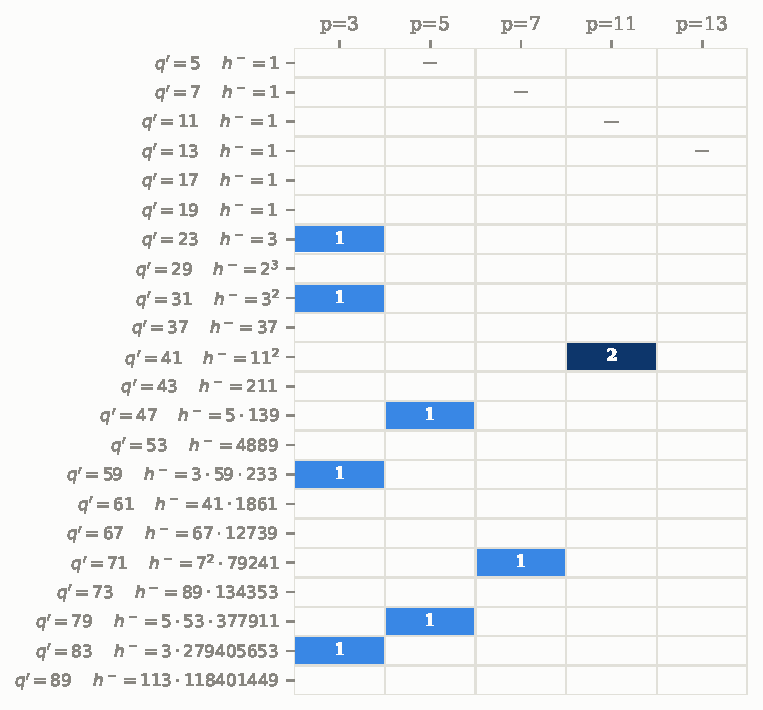
\includegraphics[width=0.72\textwidth]{fig_clase_es.pdf}
\caption{El defecto $\varphi(q')/2-W_1$ para $S=2c-q'$, sobre los primos $q'\le89$ y $p\le13$ (un guion donde $p=q'$),
con $h^-(\QQ(\zeta_{q'}))$ junto a cada fila. Las celdas no nulas son exactamente los pares con $p\mid h^-$.}
\label{fig:clase}
\end{figure}

\begin{remark}[cuadrados y rectángulos]\label{obs:comp}
Para $q'$ primo, la Proposición~\ref{prop:sinnott} es la evaluación de Carlitz y Olson del determinante de Maillet.
Para $q'$ compuesto los determinantes clásicos son cuadrados. La matriz sobre las unidades, evaluada por Tateyama y por
Wang \cite{Kuc01}, (2), se anula en cuanto algún primo sobre $q'$ se descompone en $\QQ(\zeta_{q'})/\QQ(\zeta_{q'})^+$;
los determinantes de Kučera \cite{Kuc01}, Teorema~1, combinan elementos de Stickelberger de todos los niveles
$n\mid q'$ con pesos racionales; su valor lleva factores de Euler $\prod(1-\overline\chi(\ell))$, que se anulan para
algunas elecciones de pesos, y Kučera elige pesos que dan determinantes no nulos para todo conductor. La fórmula del
índice de Girstmair \cite{Gir89} usa los conjugados de un solo número cotangente dentro del cuerpo, con factores de
ramificación explícitos. La matriz rectangular $M_{q'}$, cuyo rango sobre $\QQ$ es el de Kuribayashi \cite{Kur08},
genera $2q'\Omega$, de índice $(2q')^d/w_{q'}$ en la parte
menos del ideal de Stickelberger, que es una unidad en todo $p\nmid q'$ impar; no hace falta elegir pesos. La
Figura~\ref{fig:stickel} la muestra en acción en los valores no primos: una medición anterior sobre $984$ pares
$(q',p)$ con $3\le q'<90$, $q'\not\equiv2\pmod4$ y $p\le60$ impar, $p\nmid q'$, es ahora consecuencia de la
Proposición~\ref{prop:sinnott}.
\end{remark}

\begin{figure}[htbp]
\centering
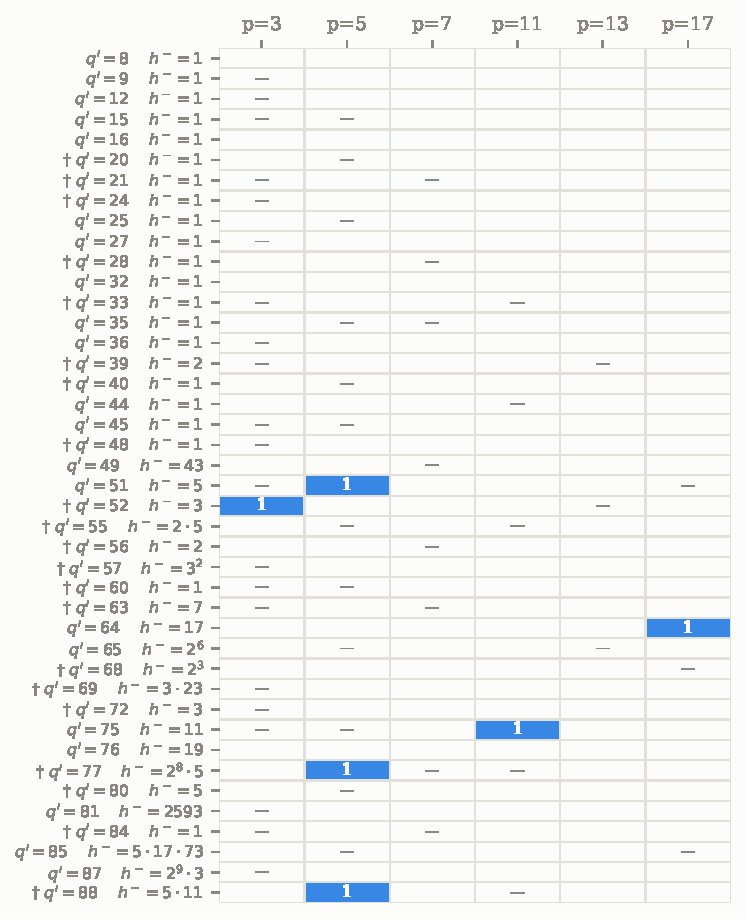
\includegraphics[width=0.74\textwidth]{fig_stickel_es.pdf}
\caption{El Teorema~\ref{thm:hminus}(a) más allá de $q'$ primo: el defecto de rango de $M_{q'}$ módulo $p$, para los
$42$ valores no primos $q'$ con $8\le q'<90$ y $q'\not\equiv2\pmod4$, y $p\le17$ (un guion donde $p\mid q'$), con el
$h^-(\QQ(\zeta_{q'}))$ exacto junto a cada fila. Las celdas no nulas son exactamente los pares con $p\mid h^-$. Una daga
marca los $21$ valores en los que la matriz cuadrada sobre las unidades sola es singular sobre $\QQ$.}
\label{fig:stickel}
\end{figure}

\noindent Un divisor simple del número de clase fija todo el cuadro local.

\begin{corollary}[un divisor simple de $h^-$]\label{cor:simple}
En el Teorema~\ref{thm:hminus}(a), supongamos que $v_p(h^-(\QQ(\zeta_{q'})))=1$. Entonces $W_1=d-1$,
\[
\marco{\cf\,\cO_p=\rad^2,\qquad v_p([\cO:A])=v_p([A:\cf])=d,}
\]
y $A_p$ es de Gorenstein.
\end{corollary}

\begin{proof}
Por la Proposición~\ref{prop:sinnott}, y el Lema~\ref{lem:dobla}(ii) cuando $q'\equiv2\pmod4$, exactamente un divisor
elemental de $M_{q'}$ es divisible por $p$, así que $W_1=d-1$ por el Teorema~\ref{thm:hminus}(a). Como $p\mid h^-$ obliga a $d\ge3$ ($h^-=1$ cuando $\varphi(q')\le20$,
\S\ref{sec:metodo}), $d/2<d-1<d$, y la Proposición~\ref{prop:mono}(b) da $e=2$;
el Teorema~\ref{thm:loc}(d) da las dos longitudes, y la Proposición~\ref{prop:gor} con $W_1=d-1$ da la propiedad de
Gorenstein.
\end{proof}

\noindent La hipótesis es suficiente, no necesaria: una potencia mayor de $p$ en $h^-$ aún puede dejar un defecto de
uno (\emph{medido}: $(q',p)=(31,3)$ y $(71,7)$, con $v_p(h^-)=2$ y rango $d-1$). \textbf{Un segundo ejemplo.} El
ejemplo guía $A_3(35)$ debe su defecto al factor en $2$, con $h^-=1$. El orden $A_{22}(69)$ lo debe al número de
clase: $q=69$, $m=22\equiv-1\pmod{23}$, $p=3$, $N=1$, $d=11$ y $h^-(\QQ(\zeta_{23}))=3$. El
Corolario~\ref{cor:simple} da $W_1=10$, $\cf\,\cO_3=\rad^2=3\cO_3$, $v_3([\cO:A])=v_3([A:\cf])=11$, y un anillo de
Gorenstein $A_{22}(69)\otimes\ZZ_3$. Un cálculo de retículo, independiente de estos argumentos, da
$[\cO:A_{22}(69)]=3^{11}$, $\cf=3\cO$, capas $(W_0,W_1,W_2,W_3)=(1,10,11,11)$ y tipo de Cohen--Macaulay $1$
(\S\ref{sec:metodo}).
Un número de clase también puede dejar un anillo que no es casi Gorenstein. Para $A_{40}(451)$ en $p=11$, con
$h^-(\QQ(\zeta_{41}))=11^2$, las capas dan $W_1=18$ y $W_2=d=20$, así que $e=2$; el anillo de multiplicadores de la
primera capa es $\FF_{11}$, $\kappa=1$, y la Proposición~\ref{prop:tipo} da tipo $2$, mientras que
$\ell(\cO_{11}/A_{11})-\ell(A_{11}/\cf\cO_{11})=21-19=2\ne\operatorname{type}-1$ (\emph{calculado} a partir de las capas,
no de un retículo).

\subsection{El diente de sierra desplazado y el factor en \texorpdfstring{$2$}{2}}\label{sec:half}

\begin{proof}[Demostración del Teorema~\ref{thm:hminus}(b)]
La fórmula de multiplicación $B_1(2x)=B_1(x)+B_1(x+\tfrac12)$ da
$\hat c/q'=B_1(\{c/q'+\tfrac12\})=B_1(\{2c/q'\})-B_1(\{c/q'\})$; sumando contra un carácter impar,
$\sum_c\chi(c)\hat c=q'(\overline\chi(2)-1)B_{1,\chi}$. Esta identidad, con el mismo factor de Euler, está en Kanemitsu y
Kuzumaki \cite{KK01}, demostración del Teorema~1 ($t=2$, módulo impar), y en Kučera \cite{Kuc01}, Ejemplo~2, donde da el
determinante de la matriz cuadrada de restos mínimos con signo; para las semisumas $\sum_{a<q'/2}\chi(a)$ véase
\cite{SUZ95}, (6). Cuando $p\nmid q'-1$ el álgebra $\FF_p[(\ZZ/q')^\times]$ es semisimple, y la dimensión del
módulo cíclico generado por la función impar $S$ es el número de caracteres impares en los que su transformada de
Fourier no se anula módulo $\mathfrak p$; la cuenta no depende de $\mathfrak p$, porque Galois permuta los
caracteres.
\end{proof}

\noindent Cuando el número de clase no interviene, el factor de Euler lo hace todo explícito, sin ninguna condición
sobre $\varphi(q')$, y también para $q'$ compuesto; lo que decide es el subgrupo $\langle2\rangle$ de $(\ZZ/q')^\times$.
Cuando ningún divisor primo de $q'$ se descompone en $\QQ(\zeta_{q'})/\QQ(\zeta_{q'})^+$ (por ejemplo, cuando $q'$ es
potencia de un primo), la parte~(a) siguiente se sigue también del determinante de Kanemitsu--Kuzumaki y Kučera
\cite{Kuc01}, (7) y Ejemplo~2, que entonces es no nulo exactamente cuando $-1\in\langle2\rangle$; la parte~(a) para los
demás $q'$ compuestos, y el rango, las longitudes y el tipo de la parte~(b), no los hemos encontrado.

\begin{corollary}[el factor en $2$]\label{cor:dos}
Sean $p$ impar, $p\mid q$, $q'\ge5$ impar, $2m+1=Nq'$ y $p\nmid N\,h^-(\QQ(\zeta_{q'}))$; sea $t$ el orden de $2$
en $(\ZZ/q')^\times$ y $d=\varphi(q')/2$.
\begin{enumerate}
\item[(a)] Si $-1\in\langle2\rangle$, entonces $W_1=d$ y $\cf\,\cO_p=\rad$.
\item[(b)] Si $-1\notin\langle2\rangle$, pongamos $\delta=d/t$. Entonces
\begin{equation}\label{eq:dos}
\marco{\begin{array}{c}W_1=d-\delta,\qquad \cf\,\cO_p=\rad^2,\\ v_p([\cO:A])=d+\delta-1,\qquad v_p([A:\cf])=d-\delta+1,\end{array}}
\end{equation}
y $A_p$ es casi Gorenstein de tipo $2\delta-1$; es de Gorenstein exactamente cuando $\delta=1$.
\end{enumerate}
\end{corollary}

\begin{proof}
Para todo resto $c$ módulo $q'$ se tiene $\hat c=\tfrac12\bigl(s_{q'}(2c)-s_{q'}(c)\bigr)$. Por tanto, con filas $u$
que recorren representantes de $(\ZZ/q')^\times/\pm1$ y columnas que recorren todos los restos,
\[
\bigl[S(u^{-1}c)\bigr]=\tfrac N2\,(P-I)\,M_{q'},
\]
donde $P$ es la matriz de permutación con signos de $u\mapsto u/2$. Como $p\nmid h^-$, la
Proposición~\ref{prop:sinnott} hace que $M_{q'}$ tenga rango $d$ módulo $p$, así que sus columnas generan
$\FF_p^d$, y el espacio de columnas de $[S(u^{-1}c)]$ es la imagen de $P-I$. La multiplicación por $2$ reparte
$(\ZZ/q')^\times/\pm1$ en órbitas. Si $-1\in\langle2\rangle$ tienen longitud $t/2$ y $P$ tiene monodromía $-1$ a lo
largo de cada una ($2^{t/2}=-1$), así que $P-I$ es invertible. Si $-1\notin\langle2\rangle$, entonces $2^ku\ne\pm u$
para $0<k<t$, así que hay $\delta$ órbitas de longitud $t$, con $t\ge3$ porque $q'\nmid2^2-1$; $P$ tiene
monodromía $+1$, y la imagen de $P-I$ es la suma directa, sobre las órbitas, de los hiperplanos $\sum\epsilon_ux_u=0$
con todos los $\epsilon_u=\pm1$. Por el Teorema~\ref{thm:loc}(b) esto da $W_1$, y (a) se sigue del
Teorema~\ref{thm:loc}(c). En (b), $t\ge3$ da $d/2<W_1<d$, así que $e=2$ por la Proposición~\ref{prop:mono}(b), y el
Teorema~\ref{thm:loc}(d) da las longitudes. Por~\eqref{eq:rango}, $V\otimes\overline{\FF}_p$ es esta suma directa de
hiperplanos reescalada coordenada a coordenada por las unidades $U_u^{-1}$; un reescalado diagonal no cambia el anillo
de multiplicadores, y los vectores $a$ con $aH\subseteq H$, para un hiperplano $H$ de $\overline{\FF}_p^{\,t}$ ($t\ge2$)
con todos los coeficientes no nulos, son las constantes. Así $\kappa=\delta$, y la Proposición~\ref{prop:tipo} da el
tipo $2\delta-1$ y la igualdad de casi Gorenstein.
\end{proof}

\noindent\textbf{El ejemplo guía, concluido.} Tomemos $q'=7$, $m=3$, $p=5$, de modo que $q=35$ y $h^-(\QQ(\zeta_7))=1$. Aquí
$2m+1=7$, y la matriz singular del \S\ref{sec:loc} la explica el carácter impar $\chi=\bigl(\frac{\cdot}{7}\bigr)$,
para el que $\chi(2)=1$ anula el factor de Euler. El
orden de $2$ módulo $7$ es $t=3$, así que $-1\notin\langle2\rangle$, $\delta=1$, y el Corolario~\ref{cor:dos}(b) da
$W_1=2$ y $e=2$. El orden de $5$
en $(\ZZ/7)^\times/\pm1$ es $3=d$, así que $5$ tiene un solo primo sobre él, con cuerpo residual $\FF_{125}$. Por el
Teorema~\ref{thm:loc}(d),
\[
\cf\,\cO_5=\rad^2,\qquad v_5([A:\cf])=1+2=3,\qquad v_5([\cO:A])=6-1-2=3 ,
\]
así que $[\cO:A_3(35)]=125$ y $[\cO:\cf]=5^6$, y por la Proposición~\ref{prop:gor} el anillo $A_3(35)\otimes\ZZ_5$ es de Gorenstein. (El cálculo de
retículos del \S\ref{sec:metodo} da los mismos números.)

\noindent\textbf{Un $\delta$ mayor.} Para $A_{15}(155)$ en $p=5$: $q'=31$, $d=15$, $t=5$, $\delta=3$ y
$h^-(\QQ(\zeta_{31}))=9$. Aquí $5\mid q'-1$, fuera del Teorema~\ref{thm:hminus}(b), pero dentro del
Corolario~\ref{cor:dos}: $W_1=12$, $\cf\,\cO_5=\rad^2$, $v_5([\cO:A])=17$, $v_5([A:\cf])=13$, y tipo $5$, así que
$A_{15}(155)\otimes\ZZ_5$ es casi Gorenstein pero no de Gorenstein. Un cálculo de retículo da
$[\cO:A_{15}(155)]=5^{17}\cdot31$, $e_5=2$, capas $(1,12,15)$ y tipo $5$ (\S\ref{sec:metodo}). El número de clase, en
cambio, puede romper la igualdad de casi Gorenstein ($A_{40}(451)$, \S\ref{sec:saw}).

\noindent\textbf{Con $q'$ compuesto.} Para $q'$ primo la condición $-1\in\langle2\rangle$ dice que $t$ es par; para $q'$
compuesto dice más. Para $q'=15$, $t=4$ pero $2^2=4\ne-1$, así que $\delta=1$: para $A_7(105)$ en $p=7$ el corolario da
$W_1=3$, $e=2$, $v_7([\cO:A])=v_7([A:\cf])=4$ y un anillo de Gorenstein, y un cálculo de retículo da
$[\cO:A_7(105)]=7^4$, capas $(1,3,4)$ y tipo $1$. Para $q'=63$, $t=6$ y $\delta=3$: el retículo de $A_{31}(315)$ en
$p=5$ tiene índice $5^{20}$, capas $(1,15,18)$ y tipo $5$, como se predice. La hipótesis sobre $h^-$ es necesaria: con
$p\mid h^-$ la predicción falla en $3$ de $7$ controles, por ejemplo $(q',p)=(77,5)$, donde $W_1=28$ y no $29$.
\emph{Medido:} las capas $W_0,W_1,W_2$ coinciden con el corolario en los $1038$ casos calculados, sobre $5\le q'<90$
impar distinto de $81$, $p\le31$ y $N\le5$, con $13$ valores compuestos de $q'$ en los que $t$ es par y
$-1\notin\langle2\rangle$; el tipo $2\delta-1$, calculado a partir de las capas, coincide en los $26$ casos calculados, con
$\delta\le4$ (\S\ref{sec:metodo}).

\noindent Los dos corolarios terminan en los mismos dos números, y el caso $W_1=d$ también. En cuanto la primera
capa está más que medio llena, el índice queda decidido.

\begin{corollary}[el índice]\label{cor:indice}
Bajo las hipótesis del Teorema~\ref{thm:loc}, supongamos $W_1>d/2$, o bien $W_1>0$ y $W_2=d$. Entonces $e\le2$ y
\[
\marco{v_p([\cO:A])=2d-1-W_1,}
\]
mientras que $v_p([A:\cf])=1$ si $W_1=d$ y $1+W_1$ si $W_1<d$. La hipótesis se cumple en las familias del
Teorema~\ref{thm:hminus}(a) en cuanto $v_p(h^-(\QQ(\zeta_{q'})))<d/2$, y allí
$v_p([\cO:A])=d-1+k$ con $k$ el número de divisores elementales de $M_{q'}$ divisibles por $p$; se cumple siempre en
el Corolario~\ref{cor:dos}, donde $v_p([\cO:A])=d-1+\delta$. Por tanto, si todo primo de $q$ o bien incumple la
condición del Teorema~\ref{thm:sop}(c) o bien satisface estas hipótesis,
\[
[\cO:A]=\prod_{p}p^{\,d_p-1+(d_p-W_1(p))},
\]
con el producto sobre los primos $p\mid q$ tales que $q'_p$ divide a $h$, $h+1$ o $h+2$, y $d_p=\varphi(q'_p)/2$.
\end{corollary}

\begin{proof}
Si $W_1=d$ entonces $e=1$ por el Teorema~\ref{thm:loc}(c) y el Teorema~\ref{thm:loc}(d) da
$v_p([\cO:A])=d-W_0=d-1$, que es $2d-1-W_1$. Si $W_1<d$ entonces $e=2$: por la Proposición~\ref{prop:mono}(b) cuando
$d/2<W_1$, y por la Proposición~\ref{prop:cert}(b) cuando $W_1>0$ y $W_2=d$. El Teorema~\ref{thm:loc}(d) da entonces
$(d-1)+(d-W_1)$ y $1+W_1$. En el Teorema~\ref{thm:hminus}(a), $d-W_1=k$ y cada uno de esos
$k$ divisores elementales aporta al menos un factor $p$ a $\Delta_{q'}$, así que $k\le v_p(\Delta_{q'})=v_p(h^-)$ por
la Proposición~\ref{prop:sinnott}, y $v_p(h^-)<d/2$ da $W_1>d/2$. En el Corolario~\ref{cor:dos},
$d-W_1=\delta=d/t$ con $t\ge3$, luego $W_1\ge2d/3$. La última fórmula es el Teorema~\ref{thm:sop}(a) y~(c), que no
dejan otros primos.
\end{proof}

\noindent \emph{Medido} contra el retículo: en los $104$ pares (orden, primo) del barrido de índices con $p$ impar,
$q'\notin\{1,2,3,4,6\}$ y $W_1>d/2$, la fórmula da el exponente del índice del retículo en todos los casos, y la
forma explícita lo da en los $103$ de ellos con $p\nmid N$ (o $p\nmid B$) y, en la familia centrada, $p\nmid h^-$;
los tres pares del barrido fuera de la hipótesis tienen todos $W_1=0$ y $p\mid N$, donde toman el relevo las
Proposiciones~\ref{prop:escalera} y~\ref{prop:descenso}. La Figura~\ref{fig:zonas} coloca los perfiles medidos sobre
el eje de la primera capa: de los $168$ con $q'\notin\{1,2,3,4,6\}$, $126$ tienen $W_1=d$ y $18$ cumplen
$d/2<W_1<d$, así que los decide la primera cláusula; los $17$ con $0<W_1\le d/2$ tienen todos $p=2$, y la segunda
cláusula decide los $10$ cuya $W_2$ está dentro del rango calculado, siempre $d$ (en los otros $7$, $E=2$, y las
longitudes del retículo son las de $e=2$); los $7$ restantes tienen $W_1=0$ (\S\ref{sec:metodo}).

\begin{figure}[htbp]
\centering
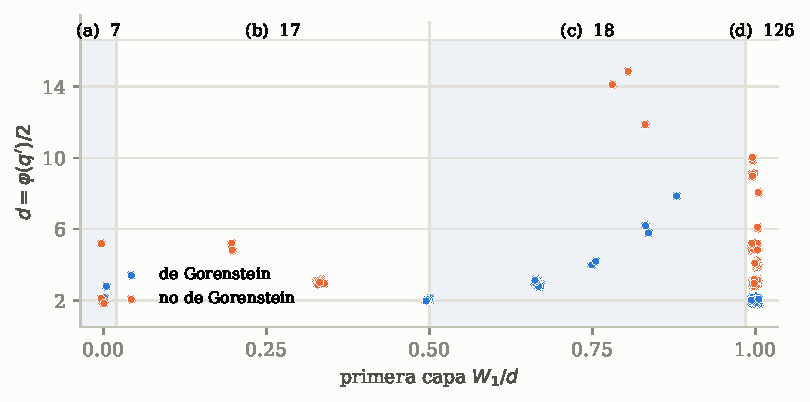
\includegraphics[width=0.86\textwidth]{fig_zonas_es.pdf}
\caption{Dónde cae la primera capa, en los $168$ perfiles medidos con $q'\notin\{1,2,3,4,6\}$, y qué decide el
exponente en cada banda: (a) $W_1=0$, la zona de la escalera y el descenso (Proposiciones~\ref{prop:escalera}
y~\ref{prop:descenso}); (b) $0<W_1\le d/2$, donde el Corolario~\ref{cor:indice} necesita su segunda cláusula
$W_2=d$; (c) $d/2<W_1<d$, donde la Proposición~\ref{prop:mono}(b) da $e=2$; (d) $W_1=d$, donde $e=1$. El color
marca si el anillo local es de Gorenstein. El eje vertical es $d=\varphi(q')/2$, con una sacudida pequeña para que
los pares repetidos se separen.}
\label{fig:zonas}
\end{figure}

\frontera{El Teorema~\ref{thm:hminus} vive en una recta de un grupo. En la recta principal de un grupo excepcional, ¿hay un orden en el que un primo que divide un número de clase relativo entra en el conductor, y qué factor de Euler hace entonces el papel de $\overline\chi(2)-1$?}

% ==============================================================================================
\section{¿Qué hay más allá de la primera capa?}\label{sec:capas}

\pregunta{La primera capa está ya ligada a los números de clase, y fija el exponente cuando está llena o llena más
de la mitad. ¿Cómo son las capas profundas?}

\noindent\textbf{Observado y certificado.} En general, una ventana finita de capas no decide el exponente:
$A_7(45)$ en $p=3$ tiene $(W_1,\dots,W_5)=(0,1,2,1,2)$ con $d=2$, así que a una capa llena le puede seguir una
deficiente; el cálculo de retículo de ese orden da $\cf\,\cO_3=\rad^5$. Llamemos \emph{exponente observado} al primer nivel a
partir del cual todas las capas calculadas están llenas. En $1183$ pares (orden, primo) cuyas capas se calcularon, la
mayoría sin cálculo de retículo ($p\le7$, $q'\le24$, $q\le260$, capas $i\le6$), los $215$ con $1\le W_1<d$ y al menos
cuatro capas calculadas tienen exponente observado $2$ (otros $34$ tienen demasiado pocas capas para decirlo). En los
$215$, la Proposición~\ref{prop:cert}(b), aplicada a los $W_1>0$ y $W_2=d$ calculados, certifica $e=2$, también en los
$10$ con varios primos sobre $p$. Lo que llena esa segunda capa es solo la estructura de anillo: \emph{medido} en
$238$ pares con $p\nmid N$, $\gr_2(A)=\gr_1(A)\cdot\gr_1(A)$, así que en grado $2$ no aparece ningún generador nuevo,
y ese producto es todo $\bar R$ en todos ellos. Pero no lo es \emph{por} ser la capa no nula: una recta estable es su
propio cuadrado salvo escalar, y la escalera produce justo eso, pues $\gr_{P-p^j}(A)$ es una recta por la
Proposición~\ref{prop:escalera}, que es la razón de que allí el exponente sea grande. Así que la hipótesis del
Corolario~\ref{cor:indice} no se puede rebajar a $\gr_1(A)\neq0$; en las familias del Teorema~\ref{thm:hminus}(a)
dice que menos de $d/2$ divisores elementales de $M_{q'}$ son divisibles por $p$, y como ese número es a lo sumo
$v_p(h^-)$, quitarla exigiría una cota del $p$-rango del grupo de clases menos. \emph{Medido}: entre $359$
subespacios estables de $\bar R$ generados por vectores al azar, con $q'\le25$ y $p\le11$, todos los de
$\dim V>d/2$ tienen por cuadrado $\bar R$, y $7$ de los $9$ con $\dim V\le d/2$ no (\S\ref{sec:metodo}).
Para $p\in\{2,3,5\}$, $q'\in\{5,7,9,11,13\}$ y capas $i\le11$, el perfil calculado
depende solo de $p$, $q'$, la familia y $v_p(N)$, y el exponente observado es a menudo, pero no siempre,
$e_0\,p^{v_p(N)}$, donde $e_0$ es el exponente observado con $v_p(N)=0$.

\begin{figure}[htbp]
\centering
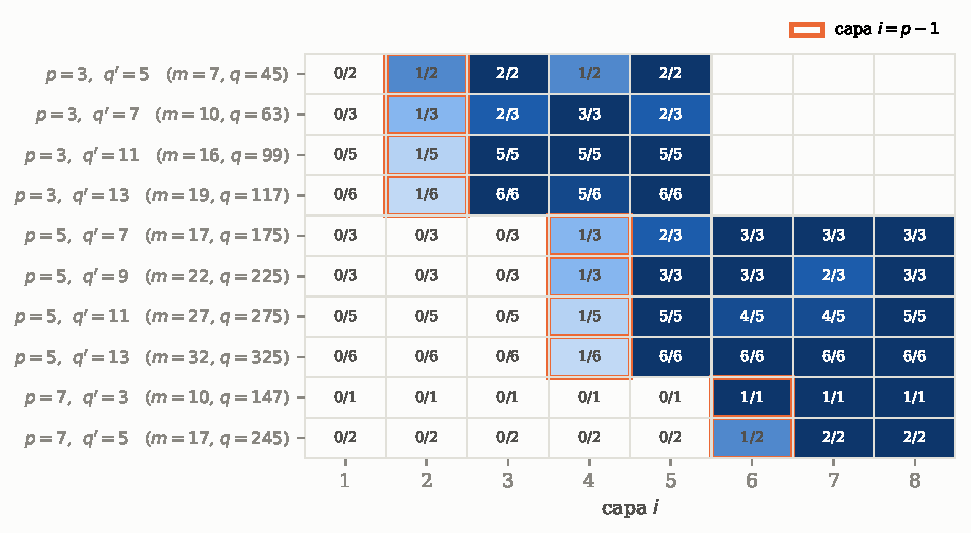
\includegraphics[width=0.86\textwidth]{fig_perfil_es.pdf}
\caption{Las capas $W_i$, escritas como $W_i/d$, para diez órdenes con $p$ impar y $v_p(N)=1$. Toda capa de grado
positivo por debajo de $p-1$ se anula y la capa $p-1$ (enmarcada) tiene dimensión $1$, como demuestra la
Proposición~\ref{prop:escalera} cuando $q'\ge5$. Solo se calcularon las capas $i<E=\varphi(p^v)$, y por eso las filas
con $p=3$ ($E=6$) se detienen en $i=5$. Las filas muestran capas, no exponentes certificados
(Proposición~\ref{prop:cert}).}
\label{fig:perfil}
\end{figure}

\noindent\textbf{Lo que la figura ya certifica.} El Corolario~\ref{cor:semigrupo} convierte algunas filas de la
Figura~\ref{fig:perfil} en exponentes sin calcular más capas. Para $A_{10}(63)$ en $p=3$ las capas son
$(1,0,1,2,3,2)$ con $d=3$: $W_2,W_3>0$ y $W_4=d$, y $\langle2,3\rangle$ contiene todo entero $\ge2$, así que toda capa
a partir de $4$ salvo quizá la $5$ está llena; $W_5=2$, así que $e=6$, $\cf\,\cO_3=\rad^6=3\cO_3$, y por la
Proposición~\ref{prop:gor} $A_{10}(63)\otimes\ZZ_3$ es de Gorenstein. Del mismo modo las filas dan $e=5$ para
$A_7(45)$, $e=3$ para $A_{16}(99)$ y $e=5$ para $A_{19}(117)$ en $p=3$, y $e=8$ para $A_{22}(225)$ y $A_{27}(275)$ y
$e=5$ para $A_{32}(325)$ en $p=5$; las filas de $A_{17}(175)$ y $A_{17}(245)$ solo acotan $e$, y $A_{10}(147)$ tiene
$q'=3$, fuera del Teorema~\ref{thm:loc}. Los cálculos de retículo
confirman los cinco valores que están a su alcance ($A_7(45)$, $A_{10}(63)$, $A_{16}(99)$, $A_{19}(117)$, $A_{22}(225)$).

\noindent La primera zona de estos perfiles no es un accidente de los ejemplos: por debajo del grado $p^{v_p(N)}$ es
universal.

\begin{proposition}[una escalera universal]\label{prop:escalera}
Sean $A\ne\ZZ$, $p$ impar, $q'\ge5$ impar, $2m+1=Nq'$ con $N=p^aM$, $a\ge1$, $p\nmid M$, y $q=p^vq'$; pongamos
$P=p^a$. Entonces $v>a$, porque $A\ne\ZZ$ obliga a $q>2m+1$ por la Proposición~\ref{prop:AZ}, es decir
$p^aM<p^v$; y $W_0=1$ y, para $1\le i<P$,
\[
\marco{W_i=\begin{cases}1,& i\in\{P-p^j:\ 0\le j<a\},\\ 0,&\text{en otro caso,}\end{cases}}
\]
En particular la primera capa no nula de grado positivo es $W_{\varphi(P)}=1$, y la imagen de $A_p$ en $\cO_p/\rad^P$
es el anillo
\[
\FF_p[\epsilon_0,\dots,\epsilon_{a-1}]/(\epsilon_i\epsilon_j:\ 0\le i,j<a),
\]
con $\epsilon_j$ en grado $P-p^j$.
\end{proposition}

\begin{proof}
Pongamos $Q_m(T)=\prod_{j=-m}^m(T-\xi^j)=(T-1)\,T^m\prod_{j=1}^m\bigl(T+T^{-1}-\eta_j\bigr)$; el paso entre los
coeficientes de $Q_m$ y las $e_k$ es triangular sobre $\ZZ$, así que generan el mismo anillo $A$. Trabajemos en
$\ZZ[\xi]$, no ramificado sobre $\cO$ encima de $p$, con $\xi=\omega\rho$, $\omega$ de orden $q'$, $\rho$ de orden $p^v$
y uniformizante $\pi=\rho-1$. Como $E=\varphi(p^v)\ge P$, las capas por debajo de $P$ solo ven la imagen de $A$ en
$\ZZ[\xi]/(p,\pi^P)=\FF_p[\omega]\otimes\FF_p[\rho]/(\rho^P-1)$, donde $\xi$ tiene orden $q'P$. Los $2m+1=Mq'P$
exponentes consecutivos recorren cada resto módulo $q'P$ exactamente $M$ veces, así que los coeficientes de $Q_m$ son
invariantes por $(\ZZ/q'P)^\times$, que actúa sobre los dos factores por separado. Los invariantes de $\FF_p[\omega]$
son $\FF_p$; los de $\FF_p[\rho]/(\rho^P-1)$ los generan las sumas sobre los subgrupos $p^j\ZZ/P$,
$\sum_{p^j\mid i}\rho^i=(\rho^P-1)/(\rho^{p^j}-1)=\pi^{P-p^j}$, $0\le j\le a$, el último de los cuales es $1$. Los
productos de los $a$ no constantes, $0\le i,j<a$, se anulan módulo $\pi^P$ porque $p^i+p^j\le2P/p<P$, lo que da la
cota superior y la estructura de anillo. Para la cota inferior tomemos un bloque,
$L=q'P$: por el teorema $q$-binomial los coeficientes de $\prod_{j=0}^{L-1}(T-\xi^j)$ son, salvo unidades,
$\genfrac{[}{]}{0pt}{}{L}{k}_\xi=\prod_{i=1}^k(1-\xi^{L-k+i})/(1-\xi^i)$. Aquí $1-\xi^i$ es una unidad salvo si $q'\mid i$,
y entonces $v_\pi(1-\xi^i)=p^{v_p(i)}$ porque $v_p(i)\le a<v$. Emparejando $i$ con $L-i$, que tienen la misma
$v_\pi(1-\xi^i)$ para $0<i<L$ (si $q'\mid i$ entonces $v_p(i)<a$), queda
$v_\pi\genfrac{[}{]}{0pt}{}{L}{k}_\xi=P-p^{v_p(k)}$ si $q'\mid k$ y $P$ en otro caso. Para $k=q'p^j$ esto es $P-p^j$.
Módulo $\pi^P$ el producto completo es la potencia $M$-ésima de un bloque desplazado, $(T^L-1+X)^M\equiv(T^L-1)^M+
M(T^L-1)^{M-1}X$, porque los coeficientes de $X$ tienen valoración al menos $P-p^{a-1}\ge P/2$; su coeficiente de
$T^{q'p^j}$ es $\pm M$ veces el de $X$, de valoración exactamente $P-p^j$, y $M$ es una unidad.
\end{proof}

\noindent Para $a=1$ esta es la observación $W_{p-1}=1$ de la Figura~\ref{fig:perfil}; para $a=2$ y $p=3$ las capas
no nulas de grado positivo por debajo de $9$ son $W_6$ y $W_8$. El primer término no nulo es a su vez un objeto
clásico: \emph{medido} en $16$ casos, todo bloque de $q'P$ exponentes consecutivos, aquí el centrado, cumple
\[
\prod_{|j|\le(q'P-1)/2}(T-\xi^j)\equiv T^{q'P}-1+\pi^{\varphi(P)}\,\mathrm{li}_1\bigl(T^{q'p^{a-1}}\bigr)
\pmod{\pi^{\varphi(P)+1}},\qquad \mathrm{li}_1(X)=\sum_{r=1}^{p-1}\frac{X^r}{r},
\]
el logaritmo finito de Kontsevich, en la notación de Besser \cite{Bes02}.

\noindent En el propio grado $p^{v_p(N)}$ vuelve la aritmética del primer momento, como primera capa de un orden menor
de la misma familia.

\begin{proposition}[descenso al segmento reducido]\label{prop:descenso}
Bajo las hipótesis de la Proposición~\ref{prop:escalera}, pongamos $m_0=(Mq'-1)/2$, $q_0=q/P$ y $A_0=A_{m_0}(q_0)$. Entonces
\[
\marco{W_P\bigl(A_m(q)\bigr)=W_1(A_0)=\dim_{\FF_p}\FF_p[(\ZZ/q')^\times]\cdot S_0,\qquad S_0(c)=M\hat c,}
\]
con ambas capas tomadas en $p$. Además, con $w=W_1(A_0)$, el anillo $A_p/(A_p\cap\rad^{P+1})$ es $\FF_p$ más un ideal de
cuadrado nulo con una base $\epsilon_0,\dots,\epsilon_{a-1},\delta_1,\dots,\delta_w$, de grados de filtración $P-p^j$ y $P$.
\end{proposition}

\begin{proof}
Mantengamos la notación de la demostración de la Proposición~\ref{prop:escalera}, con $n=q'$ y
$k=\FF_p[\omega]=\FF_p[X]/(\overline\Phi_n(X))$, $\omega=X$: un producto de $g$ copias de $\FF_{p^f}$, una por cada
primo sobre $p$, no un solo cuerpo. Escribimos $\iota$ para la involución $\omega\mapsto\omega^{-1}$ de $k$ y
$k^\pm$ para sus subespacios propios de $\pm1$, de modo que $k=k^+\oplus k^-$ porque $p\neq2$. Como
$v\ge a+1$, $E\ge2P\ge P+1$, así que $p\in\pi^{P+1}$ y $\Lambda=\ZZ_p[\xi]/(\pi^{P+1})=k[\pi]/(\pi^{P+1})$; la imagen $B$
de $A_p$ en $\Lambda$ es la $\FF_p$-álgebra generada por los coeficientes de $Q_m$, y para $i\le P$, $\gr_i(A)$ es la
imagen de $B\cap\pi^i\Lambda$ en $\pi^i\Lambda/\pi^{i+1}\Lambda=k$.

\emph{Bloques.} Pongamos $\ell=Mn=2m_0+1$ y $b=(P-1)/2$. Todo entero de $[-m,m]$ es $c+\ell j$ para exactamente un par
$|c|\le m_0$, $|j|\le b$. Con $\tau=\xi^\ell=\rho^\ell$, una raíz $p^v$-ésima primitiva de la unidad, escribamos
$\prod_{|j|\le b}(Z-\tau^j)=Z^P-1+\sum_{k=1}^{P-1}b_kZ^{P-k}$. Entonces
\begin{equation}\label{eq:bloques}
Q_m(T;\xi)=\prod_{|c|\le m_0}\bigl(T^P-\xi^{cP}+E_c(T)\bigr),\qquad E_c(T)=\sum_{k=1}^{P-1}b_k\,\xi^{ck}\,T^{P-k},
\end{equation}
y el argumento de valoraciones de la Proposición~\ref{prop:escalera}, aplicado a $\genfrac{[}{]}{0pt}{}{P}{k}_\tau$, da
$v_\pi(b_k)=P-p^{v_p(k)}\ge s:=P-P/p$, con $2s>P$. Así, módulo $\pi^{P+1}$, solo sobreviven los términos con a lo sumo un
factor $E_c$. Con $\zeta=\omega^P$, $\xi_0=\xi^P$ y $F_c(Y)=\prod_{c'\ne c}(Y-\xi_0^{c'})$,
módulo $\pi^{P+1}$
\[
[T^{Pj}]\,Q_m(T;\xi)\equiv[Y^j]\,Q_{m_0}(Y;\xi_0),\qquad
[T^{Pj+P-k}]\,Q_m(T;\xi)\equiv b_k\sum_{|c|\le m_0}\xi^{ck}\,[Y^j]\,F_c(Y).
\]

\emph{Fracciones parciales.} Sean $F(Y)=\prod_{|c|\le m_0}(Y-\zeta^c)=(Y^n-1)^M$ y $G_h=\sum_{c\in\ZZ/n}S_0(c)\zeta^{ch}$.
Agrupando los $c$ por restos, $\sum_{|c|\le m_0}\zeta^{ch}F(Y)/(Y-\zeta^c)=Mn\,(Y^n-1)^{M-1}Y^{i_h}$ con $i_h\equiv h-1$,
un polinomio entero, y $D_h(Y)=\sum_{|c|\le m_0}c\,\zeta^{ch}F(Y)/(Y-\zeta^c)=(Y^n-1)^{M-1}\sum_{i<n}G_{h-1-i}Y^i$.
Sea $V\subseteq k$ el subespacio generado por los residuos de los $G_h$; los coeficientes de todo $D_h$ están en $V$, y
los de $D_1$ en grados $n(M-1)+i$ son los $G_{-i}$, así que generan $V$. Como $S_0$ es impar, $G_h$ es antiinvariante
por $\omega\mapsto\omega^{-1}$; así $V\subseteq k^-$, mientras que $\FF_p\subseteq k^+$ y $k^+\cap k^-=0$.

\emph{El orden $A_0$.} Cumple las hipótesis del \S\ref{sec:loc} en $p$: $q_0=p^{v-a}n$ con $E_0\ge2$, $n\mid2m_0+1$,
y $2m_0<q_0$ porque $PMn\le p^vn$ y $p\nmid M$. Con $\pi_0=\rho^P-1$, $Q_{m_0}(Y;\xi_0)\equiv F(Y)-\pi_0D_1(Y)
\pmod{\pi_0^2}$, así que, exactamente como para $A_p$ arriba, $\gr_1(A_0)=V$ y $W_1(A_0)=\dim V$, que el
Teorema~\ref{thm:loc}(b) calcula como $\dim\FF_p[(\ZZ/n)^\times]\cdot S_0$.

\emph{Generadores.} Como $\pi_0\equiv\pi^P$ módulo $\pi^{P+1}$, los coeficientes en grados $Pj$ son
$[Y^j]F-\pi^P[Y^j]D_1$, con $[Y^j]F\in\ZZ$. Para $k=p^tu$, $p\nmid u$, elijamos $h$ con $Ph\equiv k\pmod n$; módulo
$\pi^{p^t+1}$ se tiene $F_c\equiv F/(Y-\zeta^c)$ y $\xi^{ck}\equiv\zeta^{ch}(1+cu\,\pi^{p^t})$. Escribiendo
$b_k=\pi^{P-p^t}\beta$ con $\beta\equiv\beta_k\in\ZZ\pmod\pi$, los coeficientes en grados $Pj+P-k$ son
$N_{k,j}\,b_k+\beta_ku\,\pi^P[Y^j]D_h$ con $N_{k,j}\in\ZZ$.

\emph{Cota inferior.} Los elementos $\pi^P[Y^j]D_1=[Y^j]F-[T^{Pj}]Q_m$ están en $B\cap\pi^P\Lambda$ con residuos que
generan $V$, así que $V\subseteq\gr_P(A)$.

\emph{Cota superior.} Todo generador está en $C=\Lambda_\rho+\pi^PV$, donde $\Lambda_\rho$ es la
imagen de $\ZZ_p[\rho]$; $C$ es un anillo, así que $B\subseteq C$, y un elemento de $C$ en $\pi^P\Lambda$ tiene su parte en
$\Lambda_\rho$ en $\FF_p\,\pi^P$. Por tanto $\gr_P(A)\subseteq\FF_p+V$, que tiene una dimensión de más.

\emph{La dirección escalar.} Quien la quita es la conjugación compleja, y aquí es donde se usa que el orden es real.
La conjugación fija $A_p$ punto a punto y envía $\pi$ a $-\pi\rho^{-1}$; como $P$ es impar, el residuo $y$ de un
elemento de $A_p\cap\rad^P$ cumple $y=-\bar y$, es decir $\gr_P(A)\subseteq k^-$, mientras que $\FF_p\subseteq k^+$ y
$k^+\cap k^-=0$ porque $p\neq2$. Así que $\gr_P(A)\subseteq(\FF_p+V)\cap k^-=V$ y, con la cota inferior,
$\gr_P(A)=V$.

\emph{Anillo.} Cada generador es un entero más un elemento de $\pi^s\Lambda$, y $2s>P$, así que los productos de estos
elementos se anulan, $B=\FF_p+\mathfrak m$ con $\mathfrak m^2=0$, y $\dim\mathfrak m=\sum_{1\le i\le P}W_i=a+w$ por
la Proposición~\ref{prop:escalera}, así que $\dim_{\FF_p}B=1+a+w$.
\end{proof}

\noindent Que el producto sea real se usa, y hace falta, en la última cota: para el producto no centrado
$\prod_{0\le x\le 2m}(T-\xi^x)$, que no es real, $\pi^P$ sí está en el álgebra de sus coeficientes módulo $\pi^{P+1}$
(\emph{medido} en cuatro casos). La proposición se cumple en los $32+953$ casos calculados, y su igualdad
$W_P=W_1(A_0)$ en otros $118$. Los $953$ recorren $p\le11$, $p^{v_p(N)}\le121$, $M\le13$ y $q'\le45$ impar distinto de
$37,41,43$, $338$ de ellos con $q'$ compuesto; se omitieron $51$ casos de esa malla por encima de una cota de coste, y un
segundo valor de $v$ solo se probó en los casos más baratos. Para $q'=7$ da el
rango $2$ del ejemplo guía, que es la caída de $W_p$ en la Figura~\ref{fig:perfil}.

\begin{question}\label{q:escalera}
La Proposición~\ref{prop:descenso} recupera, en el grado $p^{v_p(N)}$, la primera capa del orden reducido. ¿Sigue
descendiendo el perfil más allá, de modo que la capa $P+i$ de $A_m(q)$ la gobierne la capa $1+i$ de $A_{m_0}(q_0)$
corregida por la escalera, y continúa como una escalera de números de Bernoulli generalizados $B_{i,\chi}$ módulo
$\mathfrak p$, de modo que la parte $p$ de $[\cO:A]$, que por el Teorema~\ref{thm:loc}(d) es la suma de los defectos
$\sum_{i<e}(d-W_i)$, tenga una forma cerrada en términos de funciones $L$ $p$-ádicas?
\end{question}

\noindent \emph{Medido} más allá del descenso, en los $38$ pares con $p\in\{3,5,7\}$, $q'\le27$, $M\le4$ y
$v_p(N)=1$: el perfil no desciende sin más, porque la capa $P+1$ no es siempre la segunda capa de $A_0$, que por el
párrafo de arriba está siempre llena. Quien la gobierna es el momento \emph{segundo}. Con $\hat c$ el resto con signo,
el segmento de una familia centrada cumple $\sum_{|j|\le m_0,\,j\equiv c}j^2=M\hat c^{\,2}+M(M^2-1)q'^2/12$, una
función par, y $W_{P+1}$ es la dimensión del módulo cíclico sobre $\FF_p[(\ZZ/q')^\times]$ generado por
$c\mapsto\hat c^{\,2}$ en $33$ de los $38$ pares, y uno más en los $5$ restantes; mientras que $W_{P+2}=W_P$ en los
$38$. Así que el primer momento decide la primera capa y el segundo la capa que hay sobre el descenso, que es el
extremo $B_2$ de la escalera por la que pregunta la cuestión; qué añaden las $5$ excepciones, no lo sabemos
(\S\ref{sec:metodo}).

\frontera{A lo largo de la torre $q=p^vq'$ con $m=p^{v-1}q'-1$, ¿crece $v_p([\cO:A])$ como $d\,p^{v-1}$ más un término lineal en $v$, y es el coeficiente de $v$ un invariante de Iwasawa de $\QQ(\zeta_{q'p^\infty})$?}

% ==============================================================================================
\section{Conclusiones y límites}\label{sec:open}

\pregunta{¿Qué se ha demostrado, qué descansa en el trabajo de otros, qué solo se ha medido, y dónde se detiene el
método?}

\noindent\textbf{Demostrado aquí.} El soporte del conductor (Teorema~\ref{thm:sop}); su estructura local, las
longitudes como sumas de los defectos de las capas, el crecimiento y la complementariedad de las capas, y el criterio
de Gorenstein en capas (Teorema~\ref{thm:loc}, Proposiciones~\ref{prop:cert}--\ref{prop:gor}); y el vínculo entre la
primera capa y $h^-$ para $m\equiv0,-1\pmod{q'}$ con $p$ impar, $p\nmid N$ y $q'\notin\{1,2,3,4,6\}$, incluido
$q'\equiv2\pmod4$, y para las familias de medio periodo $m\equiv r,r-1\pmod{q'}$ cuando $q'\ge8$ es par, $r=q'/2$ y
$p\nmid\lceil m/r\rceil$ (Lema~\ref{lem:dobla}), con su consecuencia de que un divisor simple de $h^-$ da el cuadrado del radical en $p$ y un
anillo local de Gorenstein (Teorema~\ref{thm:hminus}, Corolario~\ref{cor:simple}); el factor en $2$ sin
semisimplicidad, para $q'$ impar primo y compuesto, con el tipo de los anillos casi Gorenstein resultantes
(Corolario~\ref{cor:dos}, Proposición~\ref{prop:tipo}); la certificación por semigrupos (Corolario~\ref{cor:semigrupo});
el índice en un primo cuya primera capa está más que medio llena (Corolario~\ref{cor:indice});
la escalera universal por debajo de $p^{v_p(N)}$ y el descenso en $p^{v_p(N)}$ (Proposiciones~\ref{prop:escalera}
y~\ref{prop:descenso}). La forma simétrica del criterio de Gorenstein, y la
desigualdad complementaria en grado $e-1$, son el caso diagonal del criterio de Campillo, Delgado y Kiyek
\cite{CDK94}, en la línea de los semigrupos de valores simétricos de Kunz \cite{Kun70,Del87}; el crecimiento de las
capas (Proposición~\ref{prop:cert}) y la desigualdad complementaria en otros grados no los hemos encontrado en esa
literatura.

\noindent\textbf{Apoyado en otros.} El lema de Amiot sobre escalas; la fórmula del índice de Sinnott en la forma de
Bernard y Kučera, de la que la Proposición~\ref{prop:sinnott} es una reformulación matricial; y la caracterización de
los anillos de Gorenstein por longitudes (Bass, Serre, Grothendieck, Herzog--Kunz, Huneke--Swanson) con su descenso; la
fórmula $\operatorname{type}+1=\dim(\mathfrak m:\mathfrak m)/\mathfrak m$ de Marseglia, de la que la
Proposición~\ref{prop:tipo} es consecuencia directa, y los anillos casi Gorenstein de Barucci y Fröberg. El rango de
$M_n$ sobre $\QQ$ es de Kuribayashi, y el factor de Euler $\overline\chi(2)-1$ del diente desplazado está en Kanemitsu y
Kuzumaki y en Kučera. No hemos encontrado un enunciado anterior de la Proposición~\ref{prop:sinnott} como fórmula para
los menores maximales de $M_n$, ni del Lema~\ref{lem:dobla}(ii) en esta forma matricial (es la relación de distribución de
$B_1$), ni del Corolario~\ref{cor:dos}(b) o de su parte~(a) fuera del Ejemplo~2 de Kučera, y no reivindicamos
prioridad sobre ninguno de ellos.

\noindent\textbf{Lo que la identificación no dice.} Para $p\nmid 2q'$ impar identifica la parte $p$ del conúcleo de la
matriz de momentos con la de $R^-/S^-$; no identifica $\cO_p/A_p$, como módulo de Galois, con un trozo del grupo de
clases. Decide la primera capa, y con ella el exponente cuando $W_1=d$ o $W_1>d/2$; por debajo de eso, el exponente
depende de capas profundas que ningún teorema de aquí calcula cuando $p\nmid N$. Cuando $v_p(h^-)\ge2$, se conoce
$v_p(\Delta_{q'})$ pero no las longitudes, ni cómo se reparten las partes $p$ de los divisores elementales, ni si ese
reparto alcanza esas capas.

\noindent\textbf{Fuera del alcance.} $q'\le2$, es decir, $q=p^v$ o $2p^v$, donde $\omega=\pm1$ y el término de primer
orden se anula; $q'\in\{3,4,6\}$, donde el Teorema~\ref{thm:sop}(b) sigue valiendo pero los enunciados del
\S\ref{sec:loc} no tienen por qué; $p=2$ en el Teorema~\ref{thm:hminus}, donde para $m\equiv0,-1\pmod{q'}$ con $N$
impar se tiene $S\equiv1$, así que $W_1=1$ sea cual sea $h^-$; $p\mid N$ (en las familias de medio periodo,
$p\mid\lceil m/r\rceil$) en el Teorema~\ref{thm:hminus}(a), y más allá del grado $p^{v_p(N)}$ en la familia
$q'\mid h+1$; la familia $q'\mid h+1$
cuando $p\mid h^-(\QQ(\zeta_{q'}))$ y o bien $q'$ es compuesto o bien $p\mid q'-1$; el tipo cuando $e\ge3$; y el índice
en un primo con $W_1\le d/2$, donde el Corolario~\ref{cor:indice} se detiene y solo hablan la escalera y el descenso.

% ==============================================================================================
\section{Cómo se calcularon los números}\label{sec:metodo}

\noindent\textbf{Órdenes.} Para cada $(m,q)$ el orden $A$ se construye en Sage como un retículo en $\cO=\ZZ[\alpha]$,
$\alpha=\xi+\xi^{-1}$, por clausura: partiendo de $\ZZ\cdot1$, el retículo se sustituye por la forma normal de
Hermite de sí mismo más sus productos por $e_1,\dots,e_m$ hasta que deja de cambiar. El punto fijo contiene a $1$ y es
estable por la multiplicación por las $e_i$, así que contiene a $\ZZ[e]$; todo elemento suyo se obtiene de $1$ mediante
tales productos y sumas, así que está contenido en $\ZZ[e]$. En $22$ casos pequeños este retículo coincide con el
que da el constructor \texttt{order} de Sage.

\noindent\textbf{Conductor e índice.} $[\cO:A]$ es el determinante de la matriz de la base en potencias de $\alpha$.
El conductor es el retículo $\{x\in\cO : x\alpha^k\in A,\ 0\le k<D\}$, $D=[K:\QQ]$, calculado como el núcleo entero de las
condiciones lineales correspondientes, y se factoriza tras maximizar solo en los primos de su norma.

\noindent\textbf{Capas.} $W_i$ se calcula sin el conductor. Sea $\Psi_n$ el polinomio mínimo de
$\zeta_n+\zeta_n^{-1}$, de grado $\varphi(n)/2$. Como $\cO=\ZZ[\alpha]$ y $\Psi_q\equiv\Psi_{q'}^{\,E}\pmod p$, para
$i<E$
\[
\cO/(p\cO+\rad^{i+1})\;\cong\;\FF_p[X]/\bigl(\overline\Psi_{q'}(X)^{i+1}\bigr),\qquad X\mapsto\alpha,
\]
y $W_i$ es la diferencia de las $\FF_p$-dimensiones de las imágenes de $A$ en dos truncaciones consecutivas,
obtenidas por álgebra lineal sobre $\FF_p$, para $q'\ge3$. (Los programas calculan esas imágenes dentro del anillo
$\ZZ[\xi]/(p,\Phi_{q'}(\xi)^{i+1})\cong\FF_p[y]/(\Phi_{q'}(y)^{i+1})$, que contiene a $\cO/(p\cO+\rad^{i+1})$ porque
$\ZZ[\xi]$ es no ramificado sobre $\cO$ encima de $p$; las dimensiones de las imágenes de $A$ son las mismas.) Las
capas $i\ge E$ requieren precisión $p$-ádica y no se calcularon de este modo. En los $184$ pares
(orden, primo del conductor) con cálculo de retículo y $e\le E$, la fórmula $v_p([A:\cf])=\sum_{i<e}W_i$ coincide con
el retículo; un par más tiene $e>E$, con $E=1$. Los $185$ pares tienen $q'\ge3$, el rango en el que vale el
isomorfismo anterior; $16$ de ellos ($q'\in\{3,4\}$ o $E=1$) quedan fuera de las hipótesis del \S\ref{sec:loc}. En los
$168$ pares dentro de ellas cuyas capas por debajo de $e$ se calcularon, los lemas del \S\ref{sec:loc} se cumplen sin
excepción, y la simetría de la Proposición~\ref{prop:gor} se cumple exactamente cuando $v_p([\cO:A])=v_p([A:\cf])$.

\noindent\textbf{Casos sintéticos} son pares (orden, primo) cuyas capas se calcularon, casi siempre sin retículo; sus
exponentes son observados, y quedan certificados mediante la Proposición~\ref{prop:cert}(b) o, donde las capas lo
permiten, el Corolario~\ref{cor:semigrupo}. Los rangos de la
Figura~\ref{fig:clase} y del Comentario~\ref{obs:comp} son rangos de matrices enteras reducidas módulo $p$. Los números
de clase relativos de los programas más antiguos se evalúan en coma flotante con la fórmula analítica del número de
clase y se redondean. Están certificados de forma independiente: para los $22$ primos de la Figura~\ref{fig:clase},
mediante un producto de normas desde cuerpos ciclotómicos en aritmética racional, y para los $66$ valores $n<90$,
$n\not\equiv2\pmod4$, mediante la misma fórmula en aritmética ciclotómica exacta en Sage, que usa la
Figura~\ref{fig:stickel}. El cálculo del grupo de clases de PARI coincide con demostración para $\varphi(n)\le20$, y
suponiendo GRH para $20<\varphi(n)\le32$. Los divisores elementales de la Proposición~\ref{prop:sinnott} se calculan
sobre $\ZZ$ y nunca se usan para calcular $h^-$.

\noindent\textbf{Qué casos, y dónde.} Los cálculos de retículo son los pares $(m,q)$ enumerados en la cabecera de cada
archivo de barrido; solo se usan los pares con resultado, y no se interpola nada. Todos los ficheros están en el directorio \texttt{conductor/} del archivo, que es plano.

\begin{center}\footnotesize
\rowcolors{2}{filaclara}{white}
\begin{tabular}{p{0.23\textwidth}p{0.36\textwidth}p{0.33\textwidth}}
\toprule
números & guion & salida \\
\midrule
órdenes, conductores, Figura~\ref{fig:paisaje} & {\ttfamily\footnotesize orden\_generado.sage, factorizar\_conductor.sage, h2\_residuo.sage; reunidos por datos\_indice.py} & {\ttfamily\footnotesize celdas\_m*\_OUT.txt, \allowbreak h2\_OUT.txt, \allowbreak r2\_OUT.txt, \allowbreak datos\_indice.json} \\
cierre $=$ orden de Sage ($22$) & {\ttfamily\footnotesize orden\_generado\_control.sage} & {\ttfamily\footnotesize orden\_generado\_control\_OUT.txt} \\
capas; $184$ pares & {\ttfamily\footnotesize perfil\_W.py, ley\_conductor.sage} & {\ttfamily\footnotesize perfil\_W\_OUT.txt, \allowbreak ley\_conductor\_ancho\_OUT.txt, \allowbreak ley\_conductor\_repro\_OUT.txt} \\
$1183$ pares, $215$ observados & {\ttfamily\footnotesize catalogo\_e.py} & {\ttfamily\footnotesize catalogo\_e\_OUT.txt} \\
$215$ certificados; lemas del \S\ref{sec:loc} en $168$ retículos & {\ttfamily\footnotesize capas\_locales.py} & {\ttfamily\footnotesize capas\_locales\_OUT.txt} \\
perfiles frente a $v_p(N)$ & {\ttfamily\footnotesize catalogo\_N.py} & {\ttfamily\footnotesize catalogo\_N\_OUT.txt} \\
Figura~\ref{fig:clase}, Teorema~\ref{thm:hminus} & {\ttfamily\footnotesize bernoulli\_W1.py, bernoulli\_2m1.py} & {\ttfamily\footnotesize bernoulli\_W1\_OUT.txt, \allowbreak bernoulli\_2m1\_OUT.txt} \\
$h^-$ exacto ($22$ primos) & {\ttfamily\footnotesize h\_menos\_exacto.py} & {\ttfamily\footnotesize h\_menos\_exacto\_OUT.txt} \\
Comentario~\ref{obs:comp} ($984$) & {\ttfamily\footnotesize rango\_compuesto.py} & {\ttfamily\footnotesize rango\_compuesto\_OUT.txt} \\
$\Psi_q\equiv\Psi_{q'}^E$; rangos por órbitas & {\ttfamily\footnotesize psi\_y\_orbitas.py} & {\ttfamily\footnotesize psi\_y\_orbitas\_OUT.txt} \\
Proposición~\ref{prop:sinnott}: $1505$ pares; $h^-$ exacto ($66$ valores) & {\ttfamily\footnotesize stickelberger\_smith.sage} & {\ttfamily\footnotesize stickelberger\_smith\_OUT.txt} \\
$h^-$ frente a PARI & {\ttfamily\footnotesize h\_menos\_pari.sage, h\_menos\_pari\_grh.sage} & {\ttfamily\footnotesize h\_menos\_pari\_OUT.txt, \allowbreak h\_menos\_pari\_grh\_OUT.txt} \\
$A_{22}(69)$ & {\ttfamily\footnotesize orden\_A22\_69.sage} & {\ttfamily\footnotesize orden\_A22\_69\_OUT.txt} \\
certificados por semigrupos; retículos $A_{19}(117)$, $A_{22}(225)$, $A_{15}(155)$ & {\ttfamily\footnotesize item1.py, lat.sage} & {\ttfamily\footnotesize item1\_OUT.txt, \allowbreak lat\_*\_OUT.txt} \\
escalera y $W_P$ ($118$); logaritmo finito ($16$) & {\ttfamily\footnotesize item2.sage, item2\_log.py} & {\ttfamily\footnotesize item2\_OUT.txt, \allowbreak item2\_log\_OUT.txt} \\
factor en $2$ ($438$) & {\ttfamily\footnotesize item3.sage, item3\_ctrl.sage} & {\ttfamily\footnotesize item3\_OUT.txt, \allowbreak item3\_ctrl\_OUT.txt} \\
tipo cuando $e=2$ ($403$) & {\ttfamily\footnotesize capas.sage, item4.sage, item4b.sage} & {\ttfamily\footnotesize item4\_OUT.txt, \allowbreak item4b\_OUT.txt} \\
descenso ($28+4$); control no centrado ($4$) & {\ttfamily\footnotesize check\_descenso.py, control.py} & {\ttfamily\footnotesize out\_batch.txt, \allowbreak out\_hminus.txt, \allowbreak control\_OUT.txt} \\
escalera y descenso ($953$) & {\ttfamily\footnotesize inst.sage, descent.sage} & {\ttfamily\footnotesize descent\_OUT\_all.txt} \\
Lema~\ref{lem:dobla}(ii): identidades, retículos ($22$), capas ($304$) & {\ttfamily\footnotesize duplicacion.py, l2r.sage} & {\ttfamily\footnotesize duplicacion\_OUT.txt, \allowbreak l2r\_OUT.txt} \\
Lema~\ref{lem:dobla}(i) ($34$); medio periodo con $4\mid q'$: capas ($158$), controles ($12$); identidad ($n\le100$), cardinal por punto medio ($98$), rango para $\ell$ general ($52$) con $7$ controles en $p=2$ & {\ttfamily\footnotesize medio.sage, cruce.sage} & {\ttfamily\footnotesize medio\_OUT.txt, \allowbreak cruce\_OUT.txt} \\
Corolario~\ref{cor:indice} contra los índices del retículo ($104$; $103$ explícitos) & {\ttfamily\footnotesize indice.sage} & {\ttfamily\footnotesize indice\_OUT.txt} \\
\S\ref{sec:capas}: segunda capa como cuadrado ($238$); más allá del descenso ($38$); subespacios estables y sus cuadrados ($359$) & {\ttfamily\footnotesize capa2.sage, cuadrado.sage} & {\ttfamily\footnotesize capa2\_OUT.txt, \allowbreak cuadrado\_OUT.txt} \\
\bottomrule
\end{tabular}
\end{center}

\begin{center}\footnotesize
\rowcolors{2}{filaclara}{white}
\begin{tabular}{p{0.23\textwidth}p{0.36\textwidth}p{0.33\textwidth}}
\toprule
números & guion & salida \\
\midrule
Corolario~\ref{cor:dos} para $q'$ impar ($1038$), controles, tipo; $A_7(105)$, $A_{31}(315)$ & {\ttfamily\footnotesize dos.sage, dos\_ctrl.sage, dos\_tipo4.sage, latchk.sage} & {\ttfamily\footnotesize dos\_OUT.txt, \allowbreak dos\_ctrl\_OUT.txt, \allowbreak dos\_tipo4\_OUT.txt, \allowbreak lat\_A7\_105\_OUT.txt, \allowbreak lat\_A31\_315\_OUT.txt} \\
instrumentos de capas contrastados entre sí & {\ttfamily\footnotesize xval\_inst.sage, xval\_inst\_dimsB.py} & {\ttfamily\footnotesize xval\_inst\_OUT.txt, \allowbreak xval\_inst\_dimsB\_OUT.txt} \\
todas las figuras & {\ttfamily\footnotesize figuras.py} & {\ttfamily\footnotesize fig\_*.pdf} \\
\bottomrule
\end{tabular}
\end{center}

% ==============================================================================================
\section*{Atribución}

\begin{center}\small
\rowcolors{2}{filaclara}{white}
\begin{tabular}{p{0.50\textwidth}p{0.42\textwidth}}
\toprule
enunciado & fuente \\
\midrule
una escala en $\ZZ/c$ con un generador coprimo distinto de $\pm$ el suyo es completa, casi completa o trivial & Amiot \cite{Ami09}, Teor.~1 \\
$A=\ZZ$ (Proposición~\ref{prop:AZ}): los puntos enteros $q\mid2m,2m+1,2m+2$ & \cite{Mar26}, Teor.~5.1; elementos racionales, Kostant \cite[Teor.~3.1]{Kostant76} \\
órdenes $\ZZ[\chi(g)]$ para grupos finitos; los primos del índice dividen a $|G|$ & Bächle--Sambale \cite{BS20}, Teor.~A, Prop.~6 \\
longitudes del conductor; Gorenstein $\iff\ell(\cO/A)=\ell(A/\cf)$ & Bass \cite[Cor.~(6.5)]{Bas63}, con el recíproco a partir de Serre y Grothendieck; Herzog--Kunz \cite{HK71}; Huneke--Swanson \cite{HS06}, §12.2 \\
forma simétrica del criterio de Gorenstein (Proposición~\ref{prop:gor}); Proposición~\ref{prop:mono} para $i+j=e-1$ & Campillo--Delgado--Kiyek \cite{CDK94}, (3.6)--(3.7) \\
descenso de la propiedad de Gorenstein; módulos canónicos & Stacks Project \cite[Tag~0BJL]{Stacks}; Bruns--Herzog \cite[Teor.~3.3.6, Prop.~3.3.18]{BH98} \\
determinante de Maillet, $D_p=\pm p^{(p-3)/2}h^-$ & Carlitz--Olson \cite{CO55}, (1.7) \\
ideal de Stickelberger y $h^-$; sus generadores e índices (Proposición~\ref{prop:sinnott}) & Sinnott \cite{Sin78,Sin80}; Bernard--Kučera \cite{BK24}; Washington \cite{Was97} \\
determinantes cuadrados para conductores compuestos; índice de cotangentes & Tateyama, Wang, Kučera \cite{Kuc01}; Girstmair \cite{Gir89} \\
rango de la matriz rectangular $M_n$ sobre $\QQ$ & Kuribayashi \cite{Kur08}; Breuer \cite{Bre00} \\
factor de Euler $\overline\chi(2)-1$ del diente desplazado; Corolario~\ref{cor:dos}(a) cuando ningún divisor primo de $q'$ se descompone en $\QQ(\zeta_{q'})/\QQ(\zeta_{q'})^+$ & Kanemitsu--Kuzumaki \cite{KK01}; Kučera \cite{Kuc01}, (7), Ej.~2 \\
tipo $+1=\dim(\mathfrak m:\mathfrak m)/\mathfrak m$; anillos casi Gorenstein & Marseglia \cite{Mars24}, Prop.~3.5, \S7.2; Barucci--Fröberg \cite{BF97} \\
logaritmo finito & Kontsevich; Besser \cite{Bes02} \\
semisumas de caracteres impares & Szmidt--Urbanowicz--Zagier \cite{SUZ95}, (6) \\
Lema~\ref{lem:galois}, Teoremas~\ref{thm:sop}, \ref{thm:loc}, \ref{thm:hminus}, Proposiciones~\ref{prop:cert}--\ref{prop:unprimo} (Proposición~\ref{prop:mono} más allá de $i+j=e-1$), Proposición~\ref{prop:tipo} (a partir de la fórmula de Marseglia), Proposiciones~\ref{prop:escalera}, \ref{prop:descenso}, Lema~\ref{lem:dobla}, Corolarios~\ref{cor:semigrupo}, \ref{cor:dos}, \ref{cor:simple} & esta nota \\
\bottomrule
\end{tabular}
\end{center}

\section*{Disponibilidad de datos}

\noindent No se usaron datos externos. Los datos computacionales ---todo número marcado como \emph{medido} u
\emph{observado}, y todas las figuras--- los generan los programas descritos en el \S\ref{sec:metodo}, que acompañan
a esta nota junto con su salida archivada.

\renewcommand{\refname}{Referencias}
\begin{thebibliography}{99}\small\raggedright\setlength{\itemsep}{0pt}\setlength{\parskip}{0pt}
\bibitem{Ami09} E.~Amiot, \emph{About the number of generators of a musical scale}, \href{https://arxiv.org/abs/0909.0039}{\texttt{arXiv:0909.0039}} (2009).

\bibitem{BF97} V.~Barucci y R.~Fröberg, \emph{One-dimensional almost Gorenstein rings}, J.~Algebra 188 (1997), 418--442, \href{https://doi.org/10.1006/jabr.1996.6837}{\texttt{doi:10.1006/jabr.1996.6837}}.

\bibitem{BK24} O.~Bernard y R.~Kučera, \emph{A short basis of the Stickelberger ideal of a cyclotomic field}, Math.~Comp.~93 (2024), 887--909, \href{https://doi.org/10.1090/mcom/3863}{\texttt{doi:10.1090/mcom/3863}}; numeración de lemas y ecuaciones como en \href{https://arxiv.org/abs/2109.13329}{\texttt{arXiv:2109.13329v1}}.

\bibitem{Bes02} A.~Besser, \emph{Finite and $p$-adic polylogarithms}, Compositio Math.~130 (2002), 215--223, \href{https://doi.org/10.1023/A:1013727116183}{\texttt{doi:10.1023/A:1013727116183}}.

\bibitem{Bre00} T.~Breuer, \emph{Characters and Automorphism Groups of Compact Riemann Surfaces}, London Math.~Soc.
Lecture Note Ser.~280, Cambridge Univ.~Press, 2000.

\bibitem{BS20} S.~B\"achle y B.~Sambale, \emph{Orders generated by character values}, Monatsh.~Math.~191 (2020), 665--678, \href{https://doi.org/10.1007/s00605-019-01324-3}{\texttt{doi:10.1007/s00605-019-01324-3}}, \href{https://arxiv.org/abs/1910.00209}{\texttt{arXiv:1910.00209}}.

\bibitem{Bas63} H.~Bass, \emph{On the ubiquity of Gorenstein rings}, Math.~Z.~82 (1963), 8--28, \href{https://doi.org/10.1007/BF01112819}{\texttt{doi:10.1007/BF01112819}}.

\bibitem{BH98} W.~Bruns y J.~Herzog, \emph{Cohen--Macaulay Rings}, ed.~revisada, Cambridge Stud.~Adv.~Math.~39, Cambridge Univ.~Press, 1998, \href{https://doi.org/10.1017/CBO9780511608681}{\texttt{doi:10.1017/CBO9780511608681}}.

\bibitem{CDK94} A.~Campillo, F.~Delgado y K.~Kiyek, \emph{Gorenstein property and symmetry for one-dimensional local Cohen--Macaulay rings}, Manuscripta Math.~83 (1994), 405--423, \href{https://doi.org/10.1007/BF02567623}{\texttt{doi:10.1007/BF02567623}}.

\bibitem{CO55} L.~Carlitz y F.~R.~Olson, \emph{Maillet's determinant}, Proc.~Amer.~Math.~Soc.~6 (1955), 265--269, \href{https://doi.org/10.1090/S0002-9939-1955-0069207-2}{\texttt{doi:10.1090/S0002-9939-1955-0069207-2}}.

\bibitem{Del87} F.~Delgado de la Mata, \emph{The semigroup of values of a curve singularity with several branches}, Manuscripta Math.~59 (1987), 347--374, \href{https://doi.org/10.1007/BF01174799}{\texttt{doi:10.1007/BF01174799}}.

\bibitem{Ded77} R.~Dedekind, \emph{\"Uber die Anzahl der Ideal-Klassen in den verschiedenen Ordnungen eines endlichen K\"orpers}, en: Festschrift der Technischen Hochschule Braunschweig zur S\"acularfeier des Geburtstages von C.~F.~Gau{\ss}, Vieweg, Braunschweig (1877), 1--55.

\bibitem{Ded78} R.~Dedekind, \emph{\"Uber den Zusammenhang zwischen der Theorie der Ideale und der Theorie der h\"oheren Congruenzen}, Abh.~K\"onigl.~Ges.~Wiss.~G\"ottingen, Math.~Cl.~23 (1878), 3--37. Traducción inglesa comentada de F.~Q.~Gouv\^ea y J.~Webster, \href{https://arxiv.org/abs/2107.08905}{\texttt{arXiv:2107.08905}}.

\bibitem{Gir89} K.~Girstmair, \emph{An index formula for the relative class number of an abelian number field}, J.~Number Theory 32 (1989), 100--110, \href{https://doi.org/10.1016/0022-314X(89)90100-5}{\texttt{doi:10.1016/0022-314X(89)90100-5}}.

\bibitem{GS19} T.~Gannon y A.~Schopieray, \emph{Algebraic number fields generated by dimensions in fusion rings}, Commun.~Number Theory Phys.~18 (2024), 705--743, \href{https://doi.org/10.4310/cntp.241202233757}{\texttt{doi:10.4310/cntp.241202233757}}; prepublicación \emph{\dots\ by Frobenius--Perron dimensions in fusion rings}, \href{https://arxiv.org/abs/1912.12260}{\texttt{arXiv:1912.12260}}.

\bibitem{HK71} J.~Herzog y E.~Kunz, \emph{Der kanonische Modul eines Cohen--Macaulay-Rings}, Lecture Notes in Math.~238, Springer, 1971, \href{https://doi.org/10.1007/BFb0059377}{\texttt{doi:10.1007/BFb0059377}}.

\bibitem{HS06} C.~Huneke e I.~Swanson, \emph{Integral Closure of Ideals, Rings, and Modules}, London Math.~Soc. Lecture Note Ser.~336, Cambridge Univ.~Press, 2006; \href{https://www.math.purdue.edu/\%7Eiswanso/book/}{copia en línea de la autora}.

\bibitem{Kostant76} B.~Kostant, \emph{On Macdonald's $\eta$-function formula, the Laplacian and generalized exponents}, Adv.~Math.~20 (1976), 179--212, \href{https://doi.org/10.1016/0001-8708(76)90186-9}{\texttt{doi:10.1016/0001-8708(76)90186-9}}.

\bibitem{KK01} S.~Kanemitsu y T.~Kuzumaki, \emph{On a generalization of the Maillet determinant II}, Acta Arith.~99 (2001), 343--361, \href{https://doi.org/10.4064/aa99-4-4}{\texttt{doi:10.4064/aa99-4-4}}.

\bibitem{Kun70} E.~Kunz, \emph{The value-semigroup of a one-dimensional Gorenstein ring}, Proc.~Amer.~Math.~Soc.~25 (1970), 748--751, \href{https://doi.org/10.1090/S0002-9939-1970-0265353-7}{\texttt{doi:10.1090/S0002-9939-1970-0265353-7}}.

\bibitem{Kuc01} R.~Ku\v{c}era, \emph{Formulae for the relative class number of an imaginary abelian field in the form of a determinant}, Nagoya Math.~J.~163 (2001), 167--191, \href{https://doi.org/10.1017/S0027763000007959}{\texttt{doi:10.1017/S0027763000007959}}.

\bibitem{Kur08} I.~Kuribayashi, \emph{A remark on the Breuer's conjecture related to the Maillet's matrix}, Tokyo J.~Math.~31 (2008), 95--110, \href{https://doi.org/10.3836/tjm/1219844825}{\texttt{doi:10.3836/tjm/1219844825}}.

\bibitem{Mars24} S.~Marseglia, \emph{Cohen--Macaulay type of orders, generators and ideal classes}, J.~Algebra 658 (2024), 247--276, \href{https://doi.org/10.1016/j.jalgebra.2024.05.051}{\texttt{doi:10.1016/j.jalgebra.2024.05.051}}.

\bibitem{Mar26} C.~Mar\'in, \emph{Integer character values on the $\rho$-line of $\Sp(2m)$}, Zenodo (2026), \href{https://doi.org/10.5281/zenodo.22683560}{\texttt{doi:10.5281/zenodo.22683560}}.

\bibitem{Sin78} W.~Sinnott, \emph{On the Stickelberger ideal and the circular units of a cyclotomic field}, Ann.~of Math.~108 (1978), 107--134, \href{https://doi.org/10.2307/1970932}{\texttt{doi:10.2307/1970932}}.

\bibitem{Stacks} The Stacks Project Authors, \emph{The Stacks Project}, Lema~47.21.9, \href{https://stacks.math.columbia.edu/tag/0BJL}{\texttt{Tag 0BJL}}.

\bibitem{Sin80} W.~Sinnott, \emph{On the Stickelberger ideal and the circular units of an abelian field}, Invent.~Math.~62 (1980), 181--234, \href{https://doi.org/10.1007/BF01389158}{\texttt{doi:10.1007/BF01389158}}.

\bibitem{SUZ95} J.~Szmidt, J.~Urbanowicz y D.~Zagier, \emph{Congruences among generalized Bernoulli numbers}, Acta Arith.~71 (1995), 273--278, \href{https://doi.org/10.4064/aa-71-3-273-278}{\texttt{doi:10.4064/aa-71-3-273-278}}.

\bibitem{Was97} L.~C.~Washington, \emph{Introduction to Cyclotomic Fields}, 2.ª ed., Grad.~Texts in Math.~83, Springer, 1997, \href{https://doi.org/10.1007/978-1-4612-1934-7}{\texttt{doi:10.1007/978-1-4612-1934-7}}.

\end{thebibliography}

\end{document}
